\documentclass{article}

\usepackage{arxiv}

\usepackage[utf8]{inputenc} % allow utf-8 input
\usepackage[T1]{fontenc}    % use 8-bit T1 fonts
\usepackage{hyperref}       % hyperlinks
\usepackage{url}            % simple URL typesetting
\usepackage{booktabs}       % professional-quality tables
\usepackage{amsfonts}       % blackboard math symbols
\usepackage{nicefrac}       % compact symbols for 1/2, etc.
\usepackage{microtype}      % microtypography
\usepackage{lipsum}
\usepackage[algoruled]{algorithm2e}
\usepackage{amsmath}
\usepackage{graphicx}
\usepackage{subcaption}
\usepackage{printlen}
\usepackage[]{natbib} %authoryear,round,longnamesfirst

\graphicspath{ {./figures/} }

\title{Tail Free Sampling for Open-Ended Neural Text Generation}

\author{
  Trenton B.~Bricken\thanks{CAN ADD EXTRA THINGS IN HERE} \\
  Duke University\\
  \texttt{trenton.bricken@duke.edu} \\
  %% examples of more authors
   \AND
  AUTHOR LIST NOT FINALIZED. \\
  %% Affiliation \\
  %% Address \\
  %% \texttt{email} \\
  %% \And
  %% Coauthor \\
  %% Affiliation \\
  %% Address \\
  %% \texttt{email} \\
  %% \And
  %% Coauthor \\
  %% Affiliation \\
  %% Address \\
  %% \texttt{email} \\
}

\begin{document}
\maketitle

\begin{abstract}

With the increasing ability for neural networks to model natural language accurately, there is likely to be a growing number of applications for open-ended neural generation tasks. Yet, recent efforts in open-ended generation have, and continue to, produce questions as to why likelihood-maximization methods such as greedy search produce degenerate outputs. This issue, and the natural exchangeablilty of words, motivates the use of stochastic, sampling based approaches. However, sampling in a way that generates both high quality and diverse outputs remains a non-trivial problem. 
\newline

In this paper, we give theoretical and empirical evidence for why existing approaches to sampling are not robust enough across generation contexts and problem domains. We propose a new sampling algorithm, Tail Free sampling, which uses the second derivative of the model's probability distribution over its tokens to ensure that only those above a certain threshold of confidence are sampled from. We show through computational and human evaluation that this results in generations that are on average of a higher quality and less degenerate that samples from other methods, namely Top-K and Nucleus sampling. This is because samples more often come from only subset of tokens that are exchangeable in a given context.

\end{abstract}

% keywords can be removed
%\keywords{First keyword \and Second keyword \and More}

\section{Introduction}

\textbf{The Problem of Maximization}
Only with the advent of deep learning has generating long, novel natural language sequences across a wide swathe of domains become desirable. These domains include: image captioning (\cite{ImageCap}), story generation (\cite{TopKandWritingPrompts}), speech synthesis (\cite{WaveNet}), and even novel antibody design (\cite{GiffordAntibody}).

Tasks requiring sequence generation exist on a spectrum between close and open-ended tasks. These differ in the degree to which there is a semantic relationship between the input provided and generation produced, with a particularly important factor being how predictable the length of the output is, given the input (\cite{BeamLengthAdjustment}). For example, more close-ended generation tasks include image captioning and machine translation. More open-ended tasks include story writing and the generation of novel protein sequences.

The failure of current likelihood-maximizing strategies such as greedy and beam search in the domain of open-ended generation by producing short, highly repetitive outputs has led to many questions, investigations, and possible explanations (\cite{Nucleus}; \cite{HUSE}; \cite{radford2019language}; \cite{BeamLengthAdjustment}; \cite{UnLikelihood}). These possible explanations have included: (i) in order to maximize information density, surprising less predictable words are used with a high frequency to avoid speaking the predictable (\cite{Nucleus}; \cite{grice1975logic}); (ii) models over-fitting to the training data (\cite{HUSE});  (iii) likelihood-maximization choosing avenues down the tree of possible generations that are dead-ends with the lowest entropy (\cite{BeamLengthAdjustment}); (iv) the cross-entropy loss used for most models lacks a term to penalize previously generated tokens (\cite{UnLikelihood}). THEY DONT ALL EXPLICITLY PUT FORWARD THIS HYPOTHESIS BUT IT CAN BE INFERRED FROM OTHER PARTS OF THE PAPER, IS IT OK TO THEN CALL THESE EXPLANATIONS?. 

\textbf{The Promise of Sampling}
It is likely that all of these ideas contribute to the difficulty of a model's highest probably outputs being of a high quality. However, one solution that addresses a number of issues with creating diverse, high quality generations, is stochastic sampling. In the domain of producing natural human language, there are often a large number of options at both the word and sentence level that convey almost the same meaning\footnote{Interestingly, this is also true of biology in the case of protein sequences where each of the 20 amino acids used to make our natural proteins are unique but they cluster in terms of their chemical properties and ability to be substituted (\cite{BLOSUM})} this motivates sampling from a set of exchangeable words, rather than choosing only the best, which represent a small subset of all possible words in a vocabulary. In addition to being theoretically sound, stochastic sampling methods are one of the most promising approaches to ensuring that generations are diverse. These produce diversity in two ways: (i) they produce diversity in the form of unique outputs that are independent from or only weakly correlated to other generated outputs because of their stochastic nature\footnote{This is particularly the case for auto-regressive models where a different token selected early on alters every the conditional probability and token sampled later.}. This is a problem with likelihood-maximization strategies that many have tried to address (\cite{BeamComparison}; \cite{DiverseBeamSearch}; \cite{IterativeBeamSearch}); (ii) sampling produces diversity in the sense of deviating from the highest probability regions of the model. \cite{HUSE} acknowledges the trade-off between generating high quality sequences that are from high probability regions of the model but may be a consequence of over-fitting, and producing sequences that represent more distant regions of probability space that can lose their quality as a result. This problem can be seen as isomorphic to the ubiquitous explore exploit trade-off and fits in with the argument for sampling from exchangeable words rather that taking only the one with the highest probability. 

\textbf{Tail Free Sampling}
While sampling is advantageous, we show that existing sampling methods fail to find the subset of exchangeable words (or tokens) at a given point in a generation. As a result they either include too few words, resulting in a loss of diversity, or too many, resulting in a loss of quality. The reason for this is because the size of the subset of exchangeable words can change dramatically given the context and existing methods are not dynamic enough to adapt to this. Rather than considering only the Top-K words at any point (\cite{TopKandWritingPrompts}) or using a fixed cumulative density function threshold (\cite{Nucleus}), we use the second derivative of the distribution over tokens to find the "tail" of the distribution, where the the tokens plateau in probability for the model to no longer consider them exchangeable. This results in a method that is more robust to both the particular generation context and problem domain and is shown to improve performance through an in depth analysis of where the tail is located and the amount token diversity created. As the ultimate task of any language generation task is to produce text that humans rate to be of a high quality, existing sampling strategies are also systematically compared between each other and tail free sampling using human evaluators. 

\section{Background and Related Work}

It has been estimated that the average human has a vocabulary of approximately ... words. Shakespeare used ... words. While we have large vocabularies, our neural architecture seems to very efficiently prune a large majority of the words in our vocabulary from our conscious consideration so that only a few, exchangeable words, are considered for use in a given context. Neural networks trained for language tasks, similarly, have a vocabulary of tokens that they can use to generate outputs from. However, modern implementations of neural networks (\cite{TopKandWritingPrompts}; \cite{radford2019language}; \cite{UnLikelihood}; \cite{XLNet}) do not prune any tokens before generation, instead assigning a probability to every token in the vocabulary. [WHY DONT THEY? WHAT ABOUT HIERARCHICAL SOFTMAX??]. This failure to prune most of the vocabulary means that many words which are not exchangeable remain to be considered for generation, and, if chosen, can significantly reduce the quality of the output. This is particularly the case for an auto-regressive model because this can derail the generation of every later token conditioned upon the bad one. This means that the probability of sampling at least one bad token and derailing a model across a sequence generation is exponential as is shown in equation (1) and \ref{fig:derailingProb}.

 ADD REFERENCE NUMBERS TO EQUATIONS 

$$P(\text{Derailed})=1-P(\text{Good Token Sampled})^{\text{Num Sampling Steps}}$$

\begin{figure}[h]
    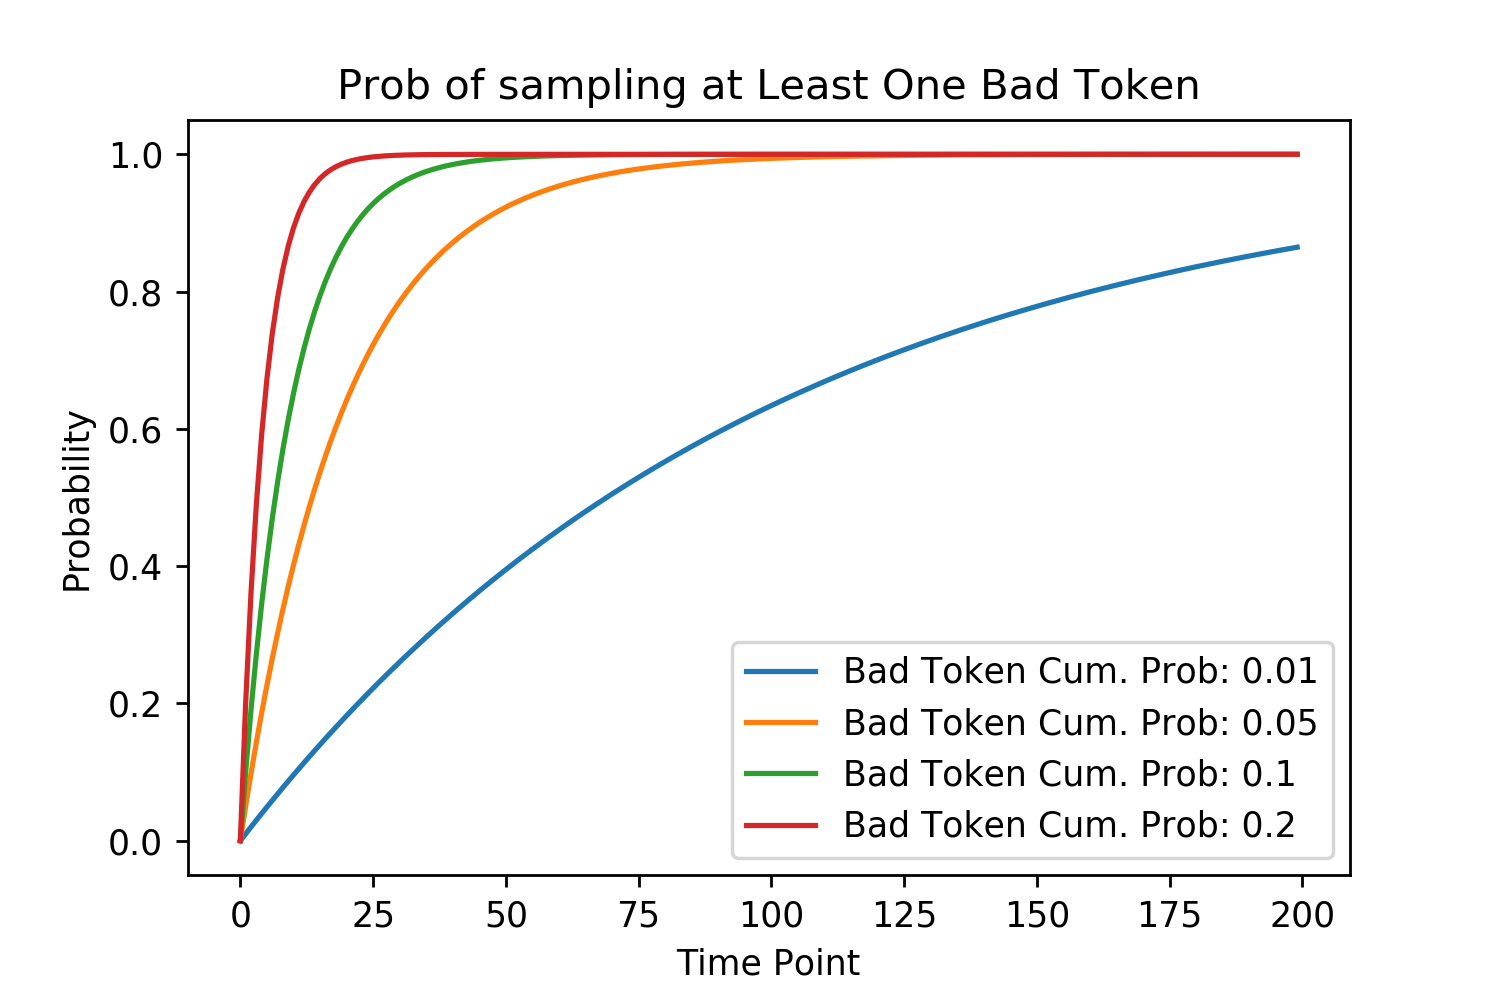
\includegraphics[width=1\textwidth]{figures/Prob_of_derailing.png}
    \caption{Each line represents a different cumulative probability that a bad token is sampled (the part of the distribution that should be pruned). This approach of sampling from the whole distribution is referred to as Ancestral sampling [cite].}
    \label{fig:derailingProb}
\end{figure}

The response to this problem has been either: (i) use likelihood-maximization; (ii) use sampling methods that prune the vocabulary. As has already been outlined in the introduction, likelihood-maximization for open-ended generation tasks results in highly repetitive, degenerate outputs. Sampling can address this problem, producing outputs that are both diverse amongst each other and represent more of the probability space. This is desirable for language because of the exchangeablility of a token subset in a particular context. 

\textbf{Current Pruning Methods for Sampling}
Top-K Sampling prunes the vocabulary by taking the highest k probability words from the distribution, normalizing them and then sampling (\cite{TopKandWritingPrompts}). [PUT IN EQUATION FOR THIS!]

However, a problem with this approach realized by \cite{Nucleus} is that at different instances, there will be fewer or more tokens that it is appropriate to select from. This is true in an absolute sense for human language, and should likewise be reflected in the relative probabilities that the model assigns to different tokens.
[SHOULD I GIVE AN EXAMPLE HERE? AND I SHOULD TAKE IT FROM THE PAPER!!]  For example, "She threw me the ..." in the context of a park could still be a ball, frisbee, apple, or many other objects. Meanwhile, ... 

This led to the introduction of Nucleus sampling, dynamically changes the threshold for pruning by using the CDF of the token probability distribution. [GIVE EQUATION]

\textbf{Motivation for Tail Free Sampling}
Tail Free Sampling (TFS) follows the same motivation for dynamically finding where to prune the distribution depending on the context of how many tokens are exchangeable. However, TFS deviates in using the second derivative of the probability distribution rather than its CDF to more accurately find the "tail" of the distribution where the tokens are no longer exchangeable. Specifically, the point at which the probabilities assigned to tokens plateaus and becomes almost uniform, indicating that the model does not predict these tokens to be worthy of any particular consideration for the context given. This application of the second derivative leads to a more robust and dynamic discovery of the model's tail as will be shown in various ways in sections ... and ... after explaining the algorithm.

\begin{figure}[h]
    \includegraphics[width=1\textwidth]{n-sampling-type_zerosevenfive_all_sps_curves}
    \caption{Sorted Probabilities for different tokens across 13,800 different generation points showing the variance in these distributions, making it difficult for Nucleus sampling to find the distribution "tail".}
    \label{fig:allDistributionCurves}
\end{figure}
%\includegraphics[width=\linewidth]{n-sampling-type_zerosevenfive_all_sps_curves.png}

Another final approach that doesn't involve explicitly pruning words but tries to achieve the same effect is by using temperature. This is applied like so... [ALGORITHM] and serves to increase or decrease the relative probabilities of tokens. [Add a plot of different temperature parameters.] This approach is also dynamic to the distribution at a particular time point. However, the temperature walks a fine line between being low enough that non exchangeable tokens are given such low probabilities they no longer threaten to derail the model and yet maintaining high enough diversity to not become a greedy optimizer. There are two reasons that temperature sampling is not further investigated in this paper. Firstly, it is not mutually exclusive to the other pruning methods and could be applied either before, after, or before and after a method that prunes. Secondly, applying a temperature to the probability distribution alters the relative probability of the tokens in a way that they no longer represent the probabilities that the model assigned to each of the tokens. This removes the location of the tail, where the probabilities plateau and the model no longer considers tokens exchangeable and can be considered a more invasive approach than that of pruning by removing the model's ability to assign calibrated confidence to its tokens.  

\begin{figure}[h]
    \includegraphics[width=1\textwidth]{TailFreeSamplingDistAdaptiveNoTitle}
    \caption{An summary of the different sampling strategies used that prune the distribution of tokens.}
    \label{fig:diffSamplingOverview}
\end{figure}

\section{Tail Free Sampling}

Most recently, \cite{UnLikelihood} have promisingly explained a component likelihood-maximization degeneration problem as being with the cross-entropy loss used for training. This has resulted in the introduction of unlikelihood training where an additional component is added to the loss function that penalizes a tokens which have been previously generated in proportion to their probability. This training method is able to increase diversity while maintaining high quality for both likelihood-maximization and sampling strategies by improving the model's probability distribution over its tokens.

NOTE HOW GENERAL THIS IS ACROSS GENERATIONS. WITH NUCLEUS THE MORE VOCAB THE DIFFERENCE IN CDF! THIS GENERALIZES ACROSS ALL MODELS AND THEIR VOCABULARY SIZE. AND THE SIZE OF THE VOCAB SHOULD NOT INFLUENCE THE NUMBER OF exchangeable WORDS, IT IS DEPENDENT UPON THE PROMPT, NOT THE MODEL IN THEORY. 
[ADD IN BETTER HEADERS AND SEGMENTATION!!!]

We define the tail of the distribution as the point at which the model’s relative probability in a particular token drops off into a plateau, beyond which point the tokens are of a sufficiently low probability. We interpret this probability dropoff as identifying tokens which can not be considered exchangeable for the current context and, therefore, should be prune.

We argue that aside from being more dynamic in finding the tail of the distribution, TFS is also more dynamic across models and problem domains with different vocabularies and contexts. The context in which a model is generating will alter the number of exchangeable words there are likely to be at any given point. Meanwhile, the size of a model's will inevitably alter its CDF. Both of these facts make Nucleus sampling and Top-K necessary to tune across models and domains while TFS with a given $z$ hyperparameter will continue to find the same tail location for the distribution.

\textbf{TFS Algorithm} The TFS algorithm is shown in \ref{alf:TFSAlgorithm} and also described step by step here. TFS first converts logits output by a model into probabilities using the softmax function before sorting them in descending order. It then calculates the first and second derivatives, as the tokens are discreet this can be found with subtraction. The magnitude of each second derivative is then taken and normalized so that they sum to 1. Finally, a threshold is used to determine what part of the cumulative distribution of the weights to define the "tail" of the distribution to be at. This is a hyperparameter that can be tuned. However, there is lower variance in the effects of this hyperparameter than for Nucleus sampling and empirically values ranging from 90\% - 95\% work well at reliably finding the last drop in the distribution before plateauing.

\begin{algorithm}[H]
    \DontPrintSemicolon
    \SetAlgoLined
    \KwIn{ Sequence of Logits, $L = (l_1, ..., l_N)$ \& CDF Threshold, $z$}
    \KwOut{ Location of the Tail, $t$ }
    $L \gets \text{sort}(L)$, where $l_i > l_2 > \ldots > l_N$ (sorting the probabilities in descending order)\;
    $L \gets \exp(l_i)/\sum_{l' \in L}{\exp(l'})$ (applying the softmax to convert logits into a probability distribution)\; 
    $D^1 \gets (l_i)_{i=2}^N - (l_i)_{i=1}^{N-1}$ (calculating the first derivative)\;
    $D^2 \gets (D^1_i)_{i=2}^N - (D^1_i)_{i=1}^{N-1}$ (calculating the second derivative)\;
    $D^2 \gets |D^2|$ (calculating the magnitude of the second derivative)\;
    $W \gets D^2_i/\sum_{d'\in D^2}{d'}$ (normalizing the second derivative)\;
    $S \gets \sum_{w' \in W}[{w'|w_{1:i-1}}]\ge z$, such that $S^{(t)} \subset W$  is the smallest set (finding the subset of CDF that surpasses the threshold)\;
    $t \gets |S|$ (getting the cardinality of the subset)\;
    \Return{$t$}
    \caption{Tail Free Sampling Algorithm, all operations are vectorized}
    \label{alg:TFSAlgorithm}
\end{algorithm}
% \ \ \    \forall i \in 1...N$\;

\begin{figure}[h]
  \begin{subfigure}{.5\textwidth}
    \centering
    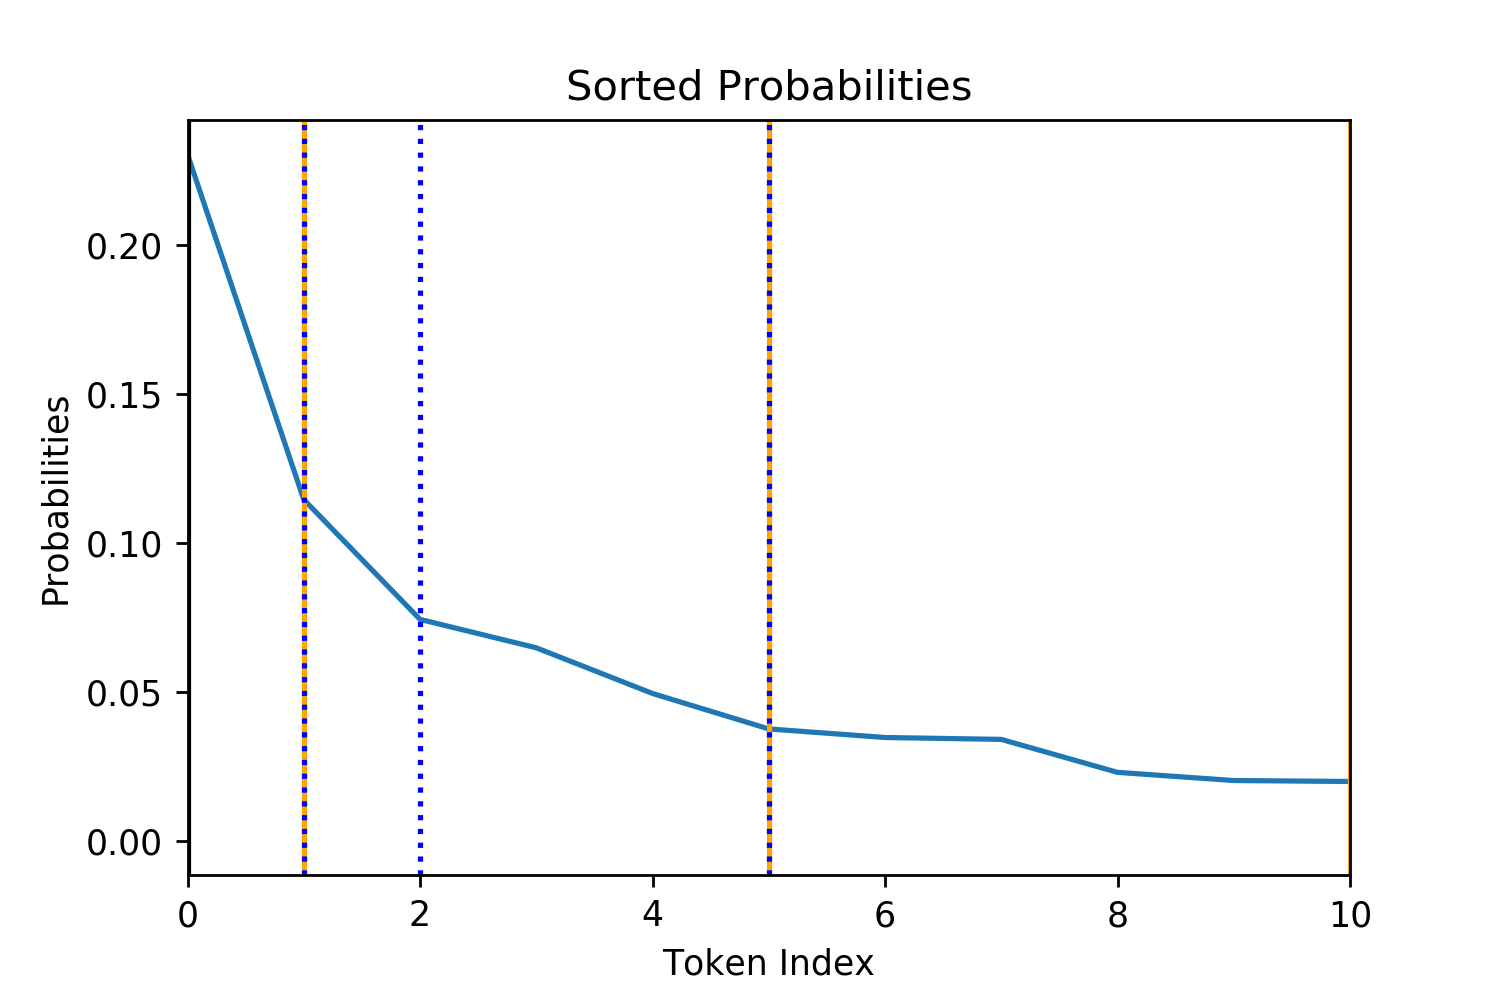
\includegraphics[width=\linewidth]{RefineTFSApproach_Algo_Explainer_Sorted_Probs}
    %\caption{Sorted Probabilities for representative logits generated from GPT-2.}
  \end{subfigure}
  \hfill
  \begin{subfigure}{.5\textwidth}
    \centering
    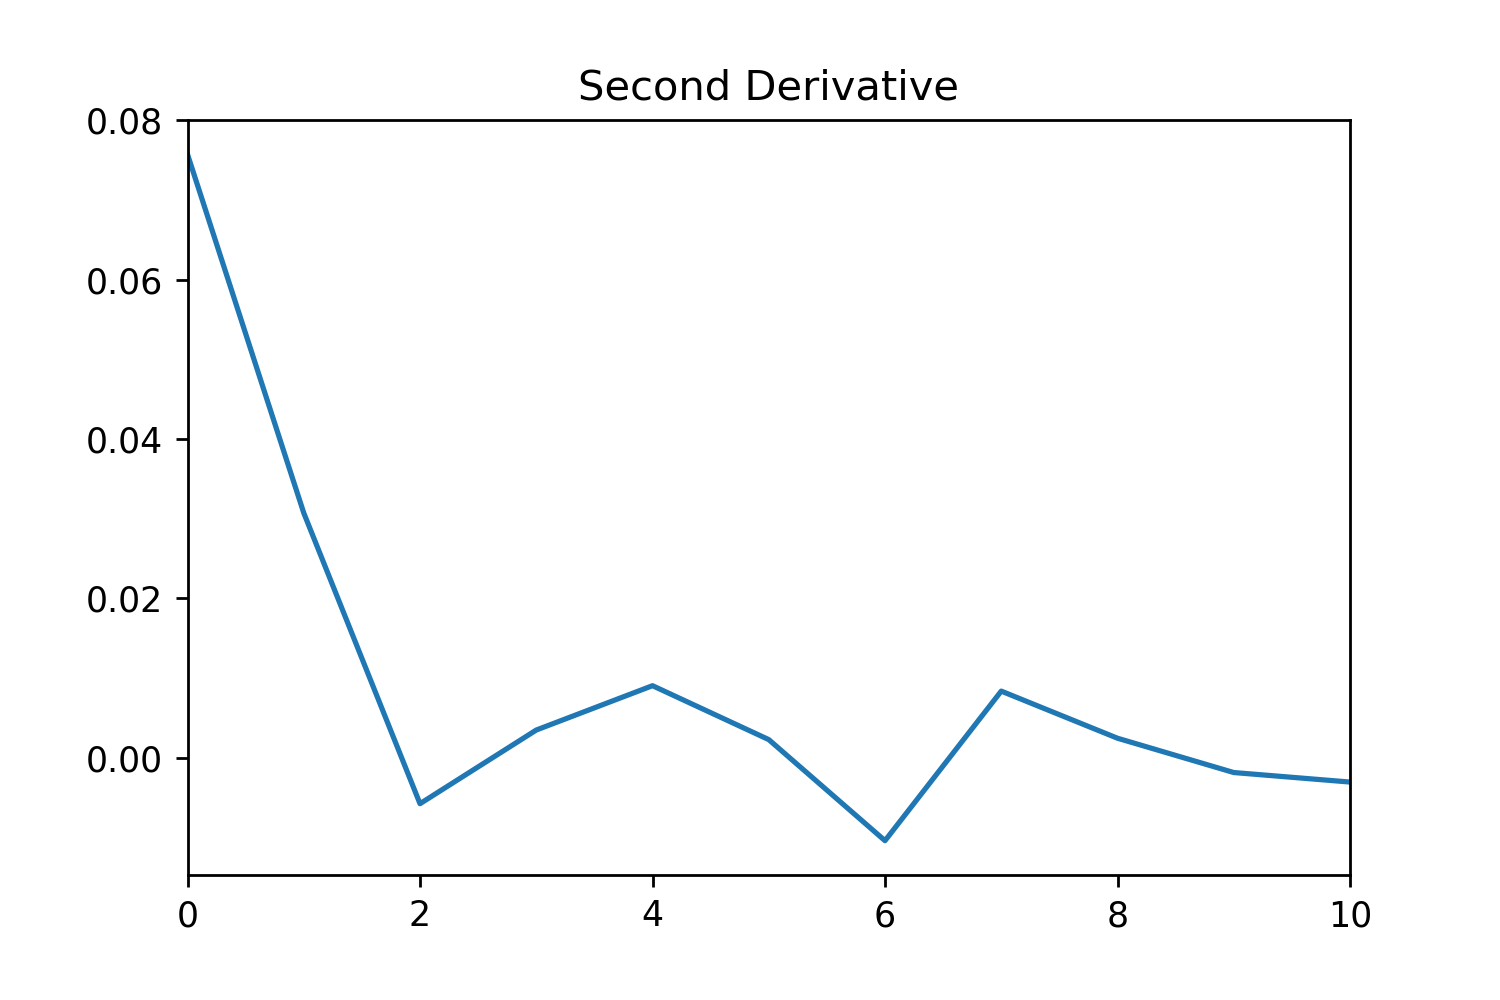
\includegraphics[width=\linewidth]{RefineTFSApproach_Algo_Explainer_Second_Der}
    %\caption{The Second Derivatives of the logits.}
  \end{subfigure}

  \medskip

  \begin{subfigure}[t]{0.5\textwidth}
    \centering
    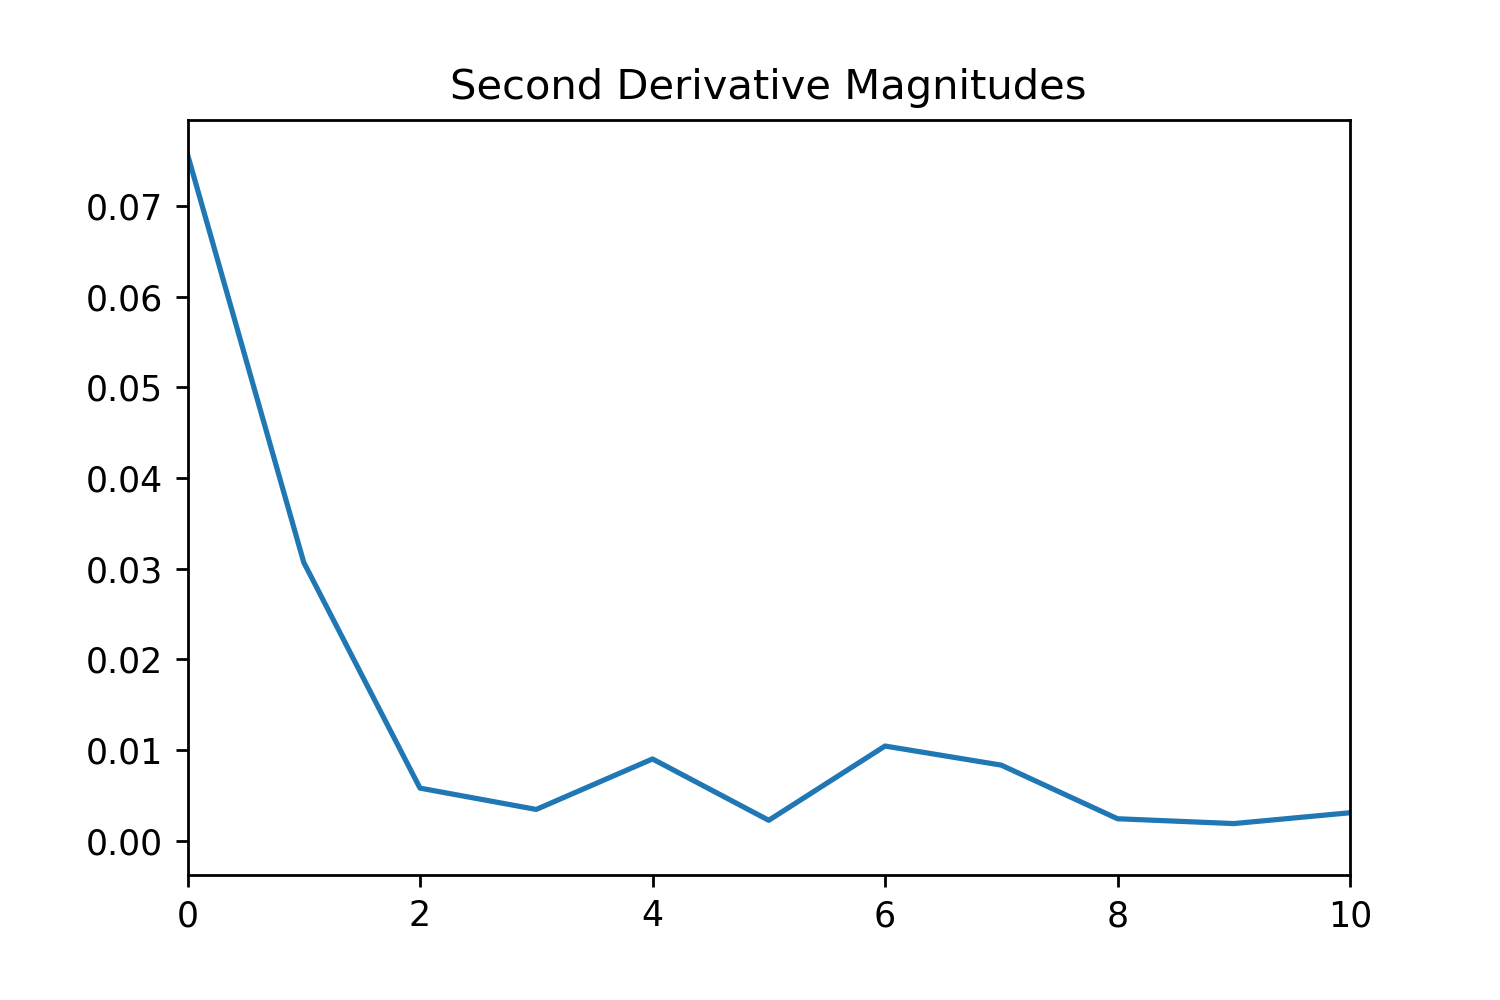
\includegraphics[width=\linewidth]{RefineTFSApproach_Algo_Explainer_Second_Der_Mags}
    %\caption{The Second derivative magnitudes.}
  \end{subfigure}
  \hfill
  \begin{subfigure}[t]{0.5\textwidth}
    \centering
    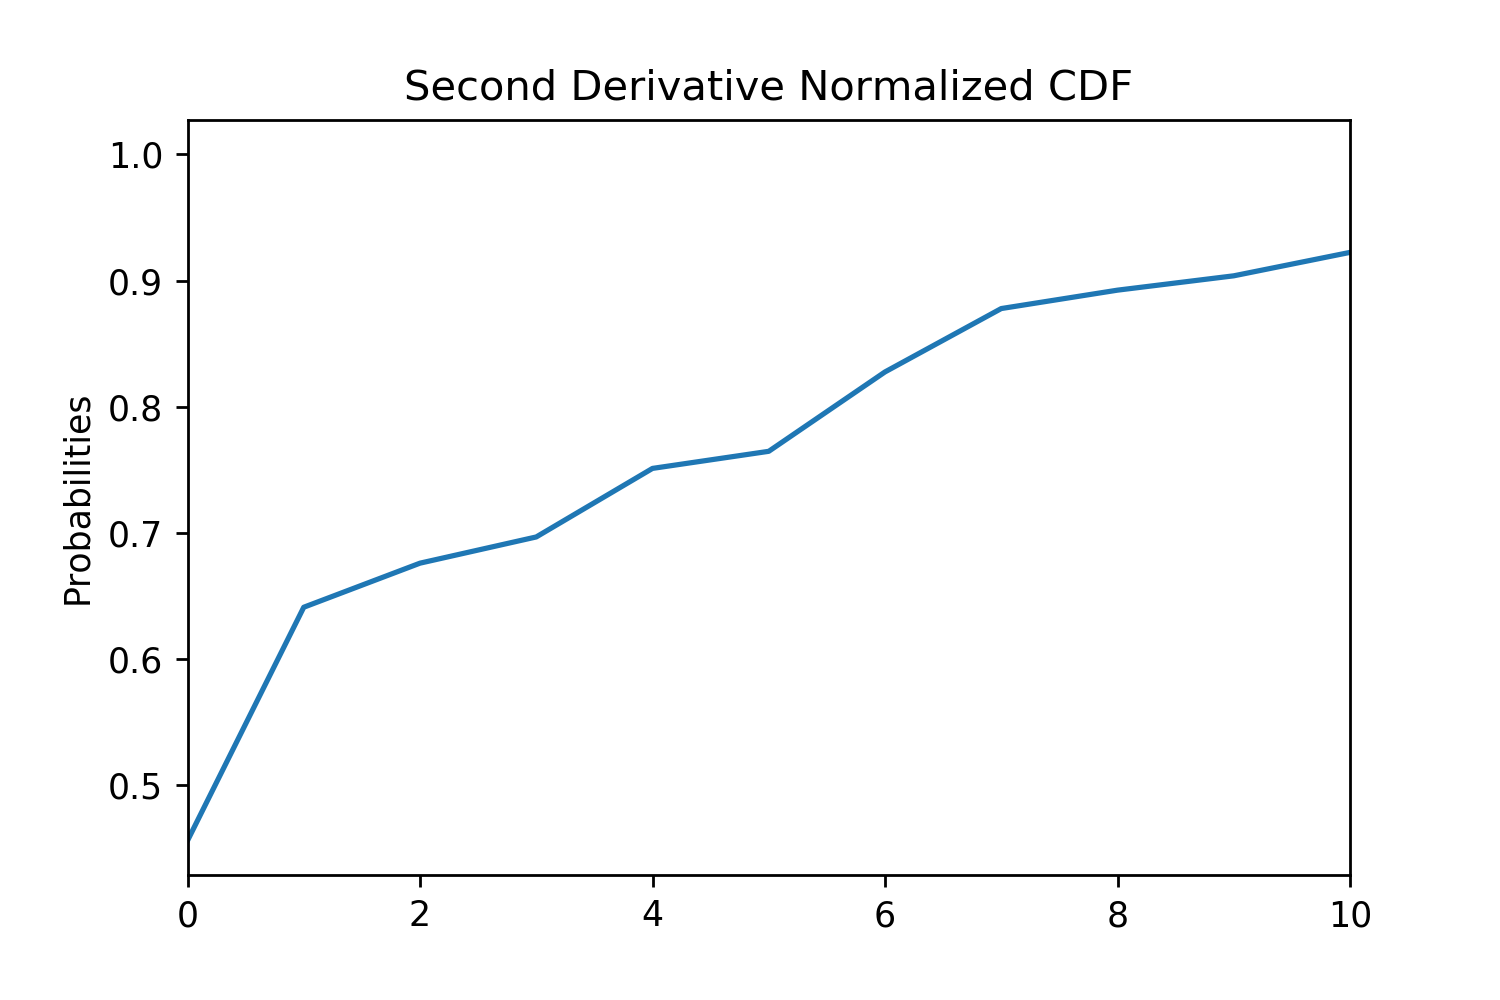
\includegraphics[width=\linewidth]{RefineTFSApproach_Algo_Explainer_Second_Der_CDF}
    %\caption{The Second Derivatives cumulatively summed. A threshold is used to determine at what point to place the tail.}
  \end{subfigure}
  \caption{Example steps in the Tail Free Sampling (TFS) algorithm using example logits generated from GPT-2. }
  \label{fig:TFSApproachExplainer}
\end{figure}

\section{Experiments}

NEED TO SAY IF I AM USING GROVER!

\textbf{Model Architecture} In order to validate the TFS algorithm, we used GPT-2's largest publicly available pretrained model with 345 million parameters (\cite{radford2019language}) \footnote{only the largest model of the \cite{radford2019language} paper with 1.5 billion parameters is officially called GPT-2, however for convenience the GPT 345M model will be referred to as GPT-2 for the rest of the paper}. No additional training of the model was performed.  

\textbf{Dataset} The probabilities for each token were generated using the same Word Prompts database (\cite{TopKandWritingPrompts}) that Nucleus sampling used which was scraped from Reddit's ... channel. Posts in this channel consist of a user writing a creative story prompt such as "[WP] A man finally discovers his superpower... well into his 80's." which other users then write short stories in response to. The dataset is presented as a pair of a prompt and human written creative short story response. 

\textbf{Text Generation} In order to compare the different sampling strategies, 100 prompts were randomly selected from the writing prompts test set. Using GPT-2's encoding, 100 tokens from the story prompt and start of the human writing were given as the starting point for GPT-2 which was then allowed to continue the story for another 150 tokens\footnote{These prompt and generation lengths are similar to those in other open-endeed generation papers (\cite{TopKandWritingPrompts}; \cite{Grover})}. First, in order for none of the sampling strategies to influence the generation and probability distributions, the human written context was given to the model at each time point. For later assessments by human evaluators and of token diversity, the same prompts were used but each sampling strategy was run using a number of different hyperparameters. GPT-2 has a vocabulary size of 50527 and at all 150 time points for all 100 prompts every logit was stored for analysis by the different sampling methods to see how each would prune the distribution. Eight of the prompts randomly selected did not have 150 tokens in the human completion of their stories and were removed for this reason leaving 92 generations for further analysis, resulting in 13,800 different sampling steps.

\subsection{Evaluation Metrics}

SAY IF I AM USING GROVER! ESP FOR THE HUMAN GENERATED EVALUATIONS.

The evaluation metrics used are briefly described here and more in depth in the Results section. Each evaluation used the Top-K, Nucleus, and TFS sampling strategies for a number of different hyperparameter values, in particular ones that seemed to be the best baselines against TFS from the analysis itself and existing literature. The evaluations used are: (i) the locations of the "tail" for each sampling method. A comparison of different tails and the CDFs of the probability distribution that they retain are analyzed; (ii) the token diversity of each sampling strategy is calculated and compared to that of the human text; (iii) MAY NOT STILL HAVE THIS the model perplexity and probability assigned to its highest probability token are assessed; (iv) the computational time that each method requires was recorded; (v) text completions were generated and evaluated in head to head comparisons by crowdsourced workers.

\section{Results}

\textbf{Tail Locations}
Five different TFS hyperparameters for $z$, determining what CDF of the second derivative cutoff were evaluated. In \ref{fig:DiffTFSCuts} we show how these different $z$ values change where the tail is identified along the token probability distribution's created by the human text completion. We decide that $z=0.95$ is a good value for relibably finding the tail and use it for our further investigations. While Nucleus sampling prunes the token distribution such that the CDF remaining equals $p+P(\text{next largest token})$, TFS pruning produces a mean CDF but that varies significantly as shown by \ref{fig:DiffTFSCDF}. The TFS where $z=0.95$ yields an average CDF threshold of 0.69 which motivated the use of Nucleus sampling with $p=0.69$ as the most similar baseline.  

\begin{figure}[h]
  \begin{subfigure}{.5\textwidth}
    \centering
    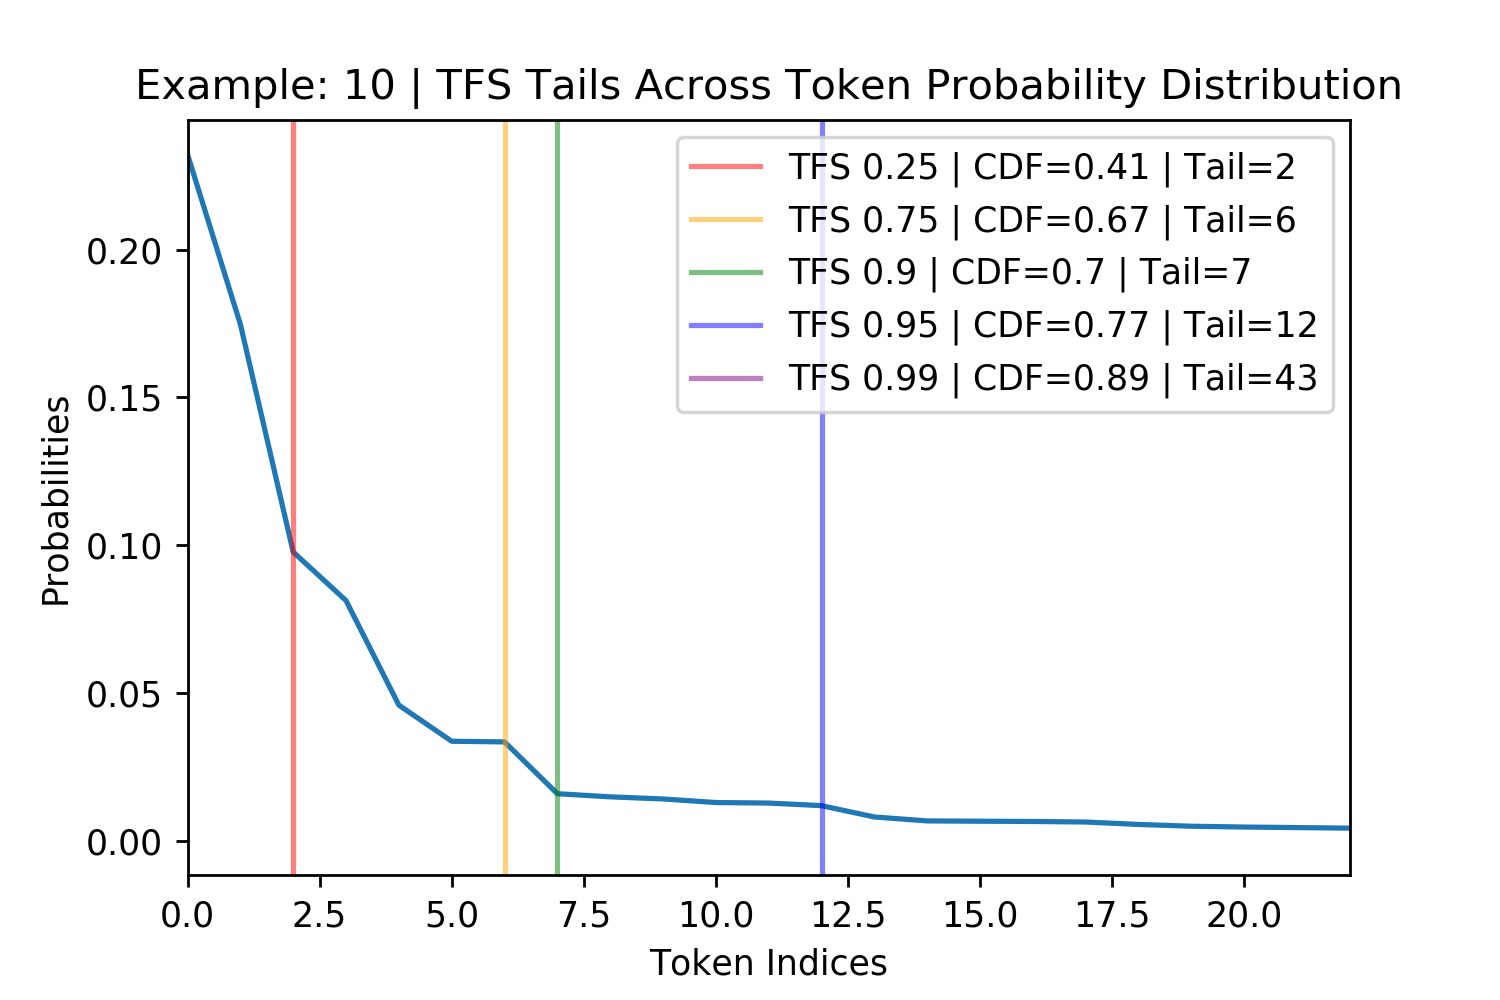
\includegraphics[width=\linewidth]{figures/Different_TFS_Values_example-9.png}
    %\caption{Sorted Probabilities for representative logits generated from GPT-2.}
  \end{subfigure}
  \hfill
  \begin{subfigure}{.5\textwidth}
    \centering
    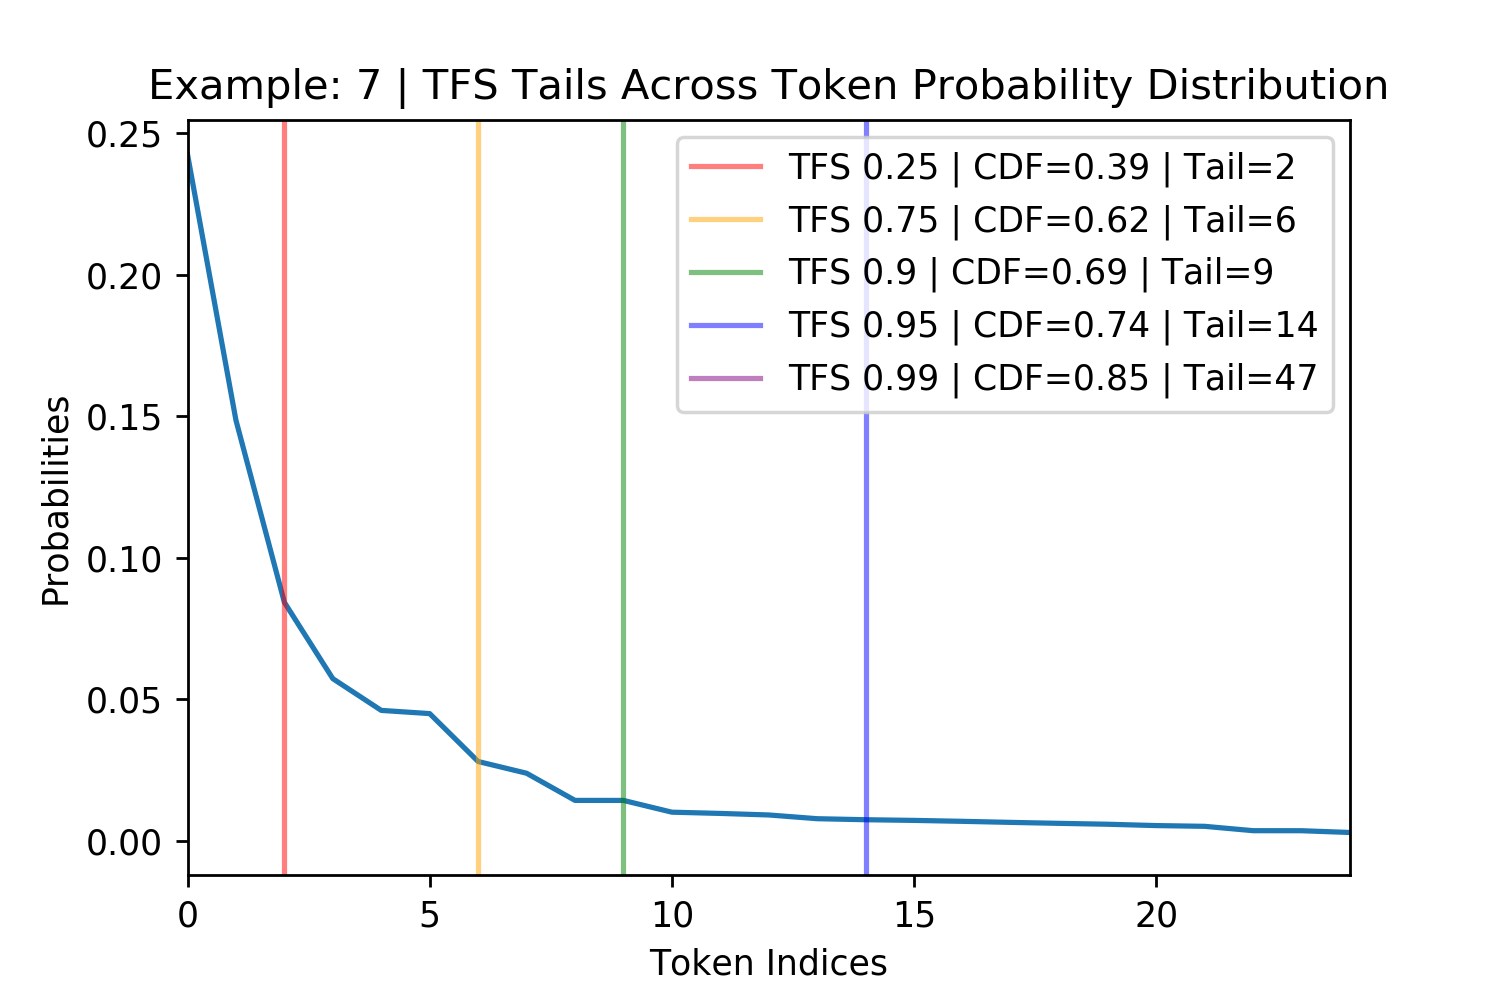
\includegraphics[width=\linewidth]{figures/Different_TFS_Values_example-6.png}
    %\caption{The Second Derivatives of the logits.}
  \end{subfigure}

  \medskip

  \begin{subfigure}[t]{0.5\textwidth}
    \centering
    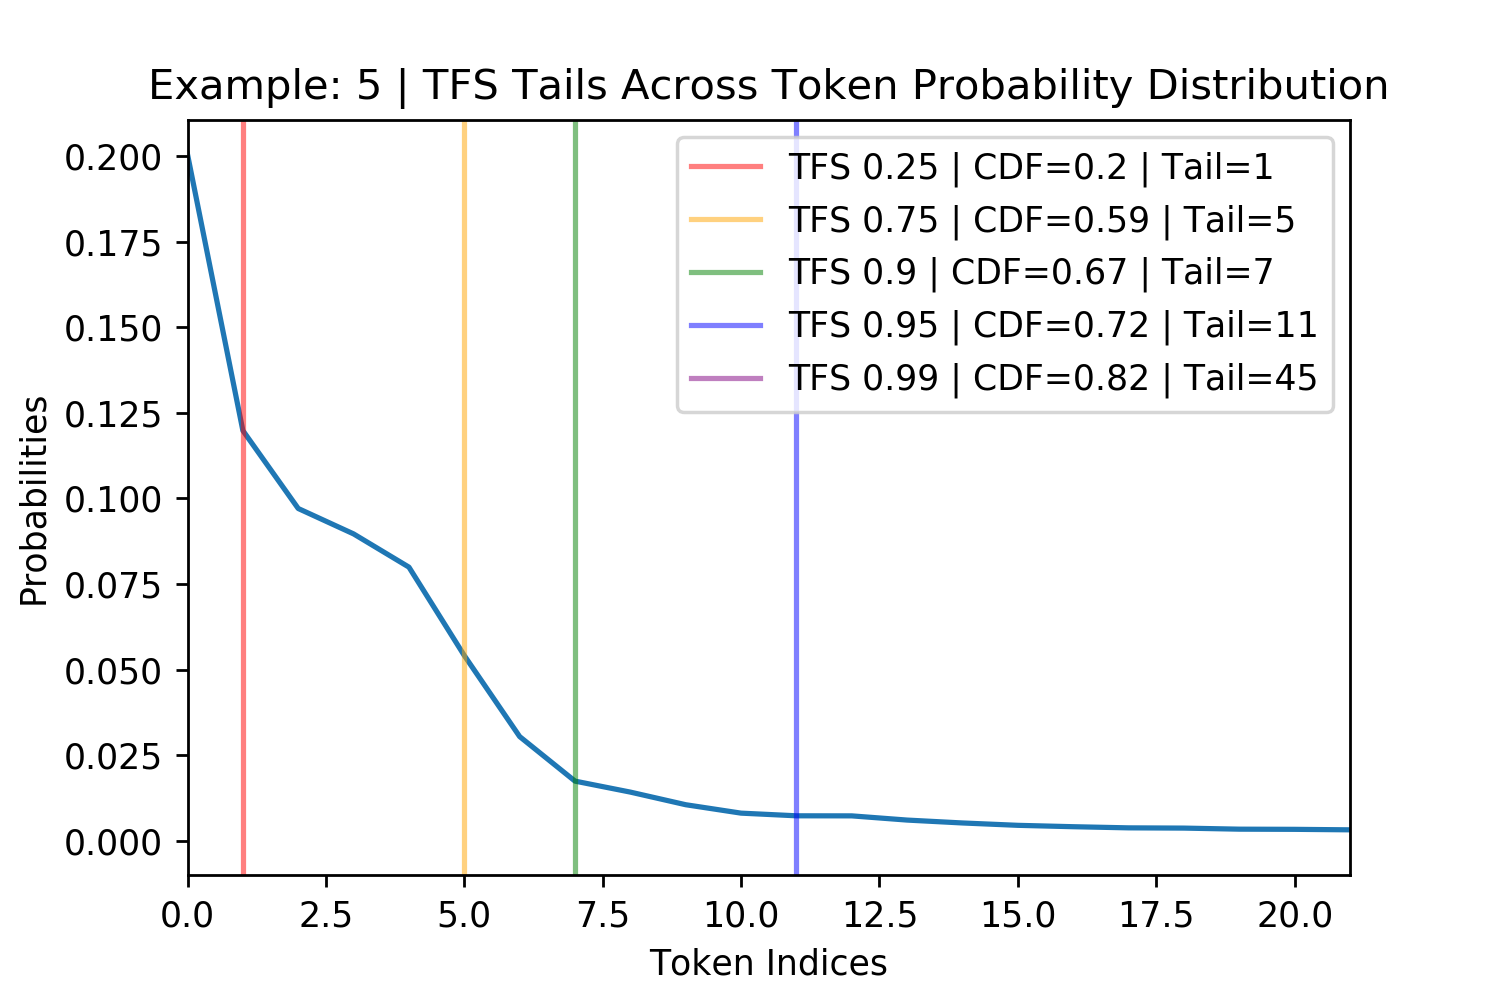
\includegraphics[width=\linewidth]{figures/Different_TFS_Values_example-4.png}
    %\caption{The Second derivative magnitudes.}
  \end{subfigure}
  \hfill
  \begin{subfigure}[t]{0.5\textwidth}
    \centering
    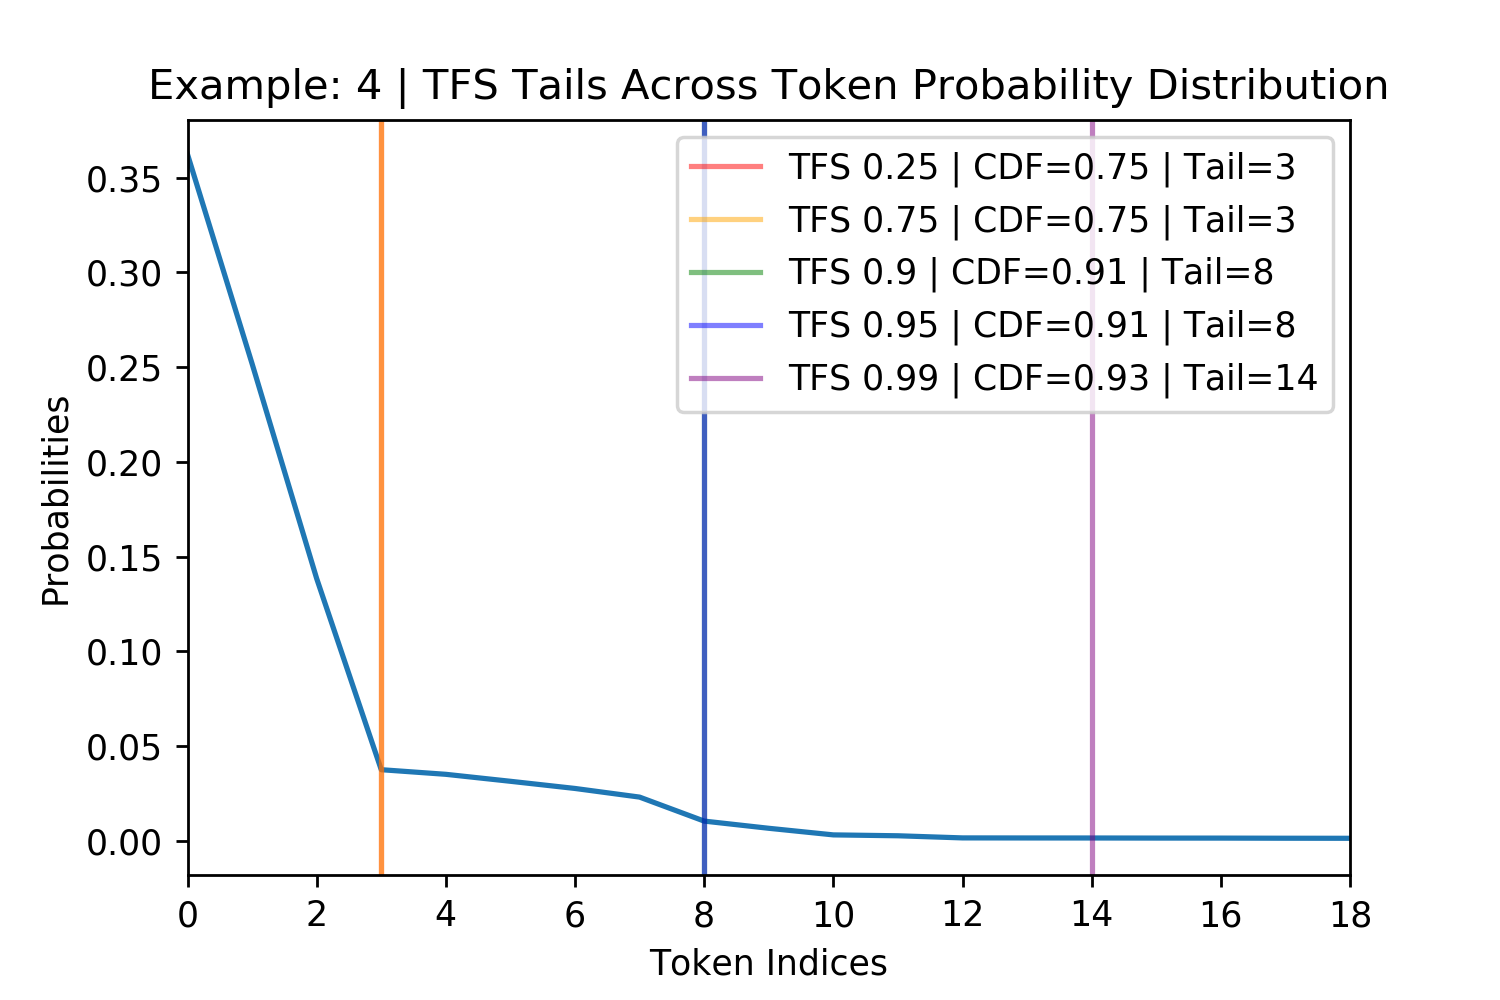
\includegraphics[width=\linewidth]{figures/Different_TFS_Values_example-3.png}
    %\caption{The Second Derivatives cumulatively summed. A threshold is used to determine at what point to place the tail.}
  \end{subfigure}
  \caption{Four randomly chosen token probability distributions out of the 13,800 possible options demonstrating how different $z$ thresholds change where the tail location is identified. The $z=0.99$ threshold does not always appear in the plot and the other thresholds sometimes overlap such as in the bottom right plot.}
  \label{fig:DiffTFSCuts}
\end{figure}

\begin{figure}[h]
    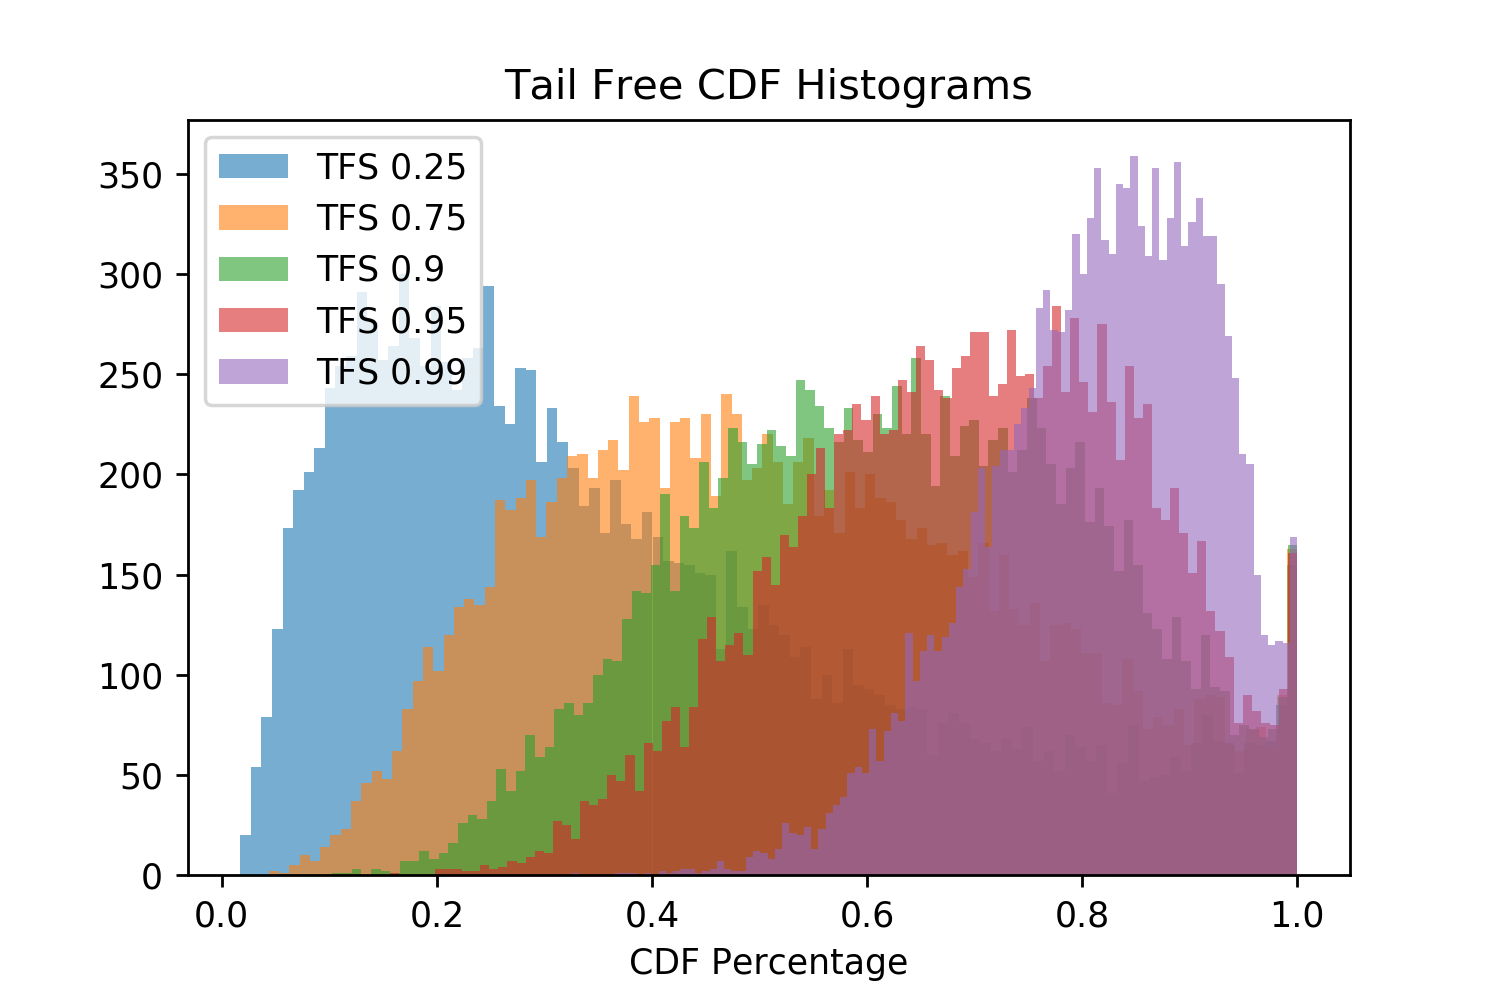
\includegraphics[width=1\textwidth]{figures/TFS_multi_cdf_in_body_hists.png}
    \caption{TFS is used to find the tail of the distribution, the CDF of the distribution that is inside the tail and will remain after pruning is calculated and histograms of 13,800 results are plotted for the different thresholds. None of the TFS's has a constant CDF threshold used to find the tail.}
    \label{fig:DiffTFSCDF}
\end{figure}

We first investigate the differences in the tail location and CDF retained for the TFS $z=0.95$ and Nucleus $p=0.69$, shown in \ref{fig:DiffTFSvsNucScatter}. Overall, ~15\% of the 13,800 sampling steps agree (this is shown as the black dotted line and can be seen most clearly in \ref{fig:DiffTFSvsNucScatter}(a). These agreements are most often where the first few tokens have disproportionately large probabilities, causing Nucleus to exceed its CDF threshold and creating a strong second derivative signal for TFS. In ~48\% of cases TFS has a tighter tail and CDF location with the remaining ~38\% Nucleus being tighter. 

\begin{figure}[h]
 
	    \begin{subfigure}{0.5\textwidth}
	    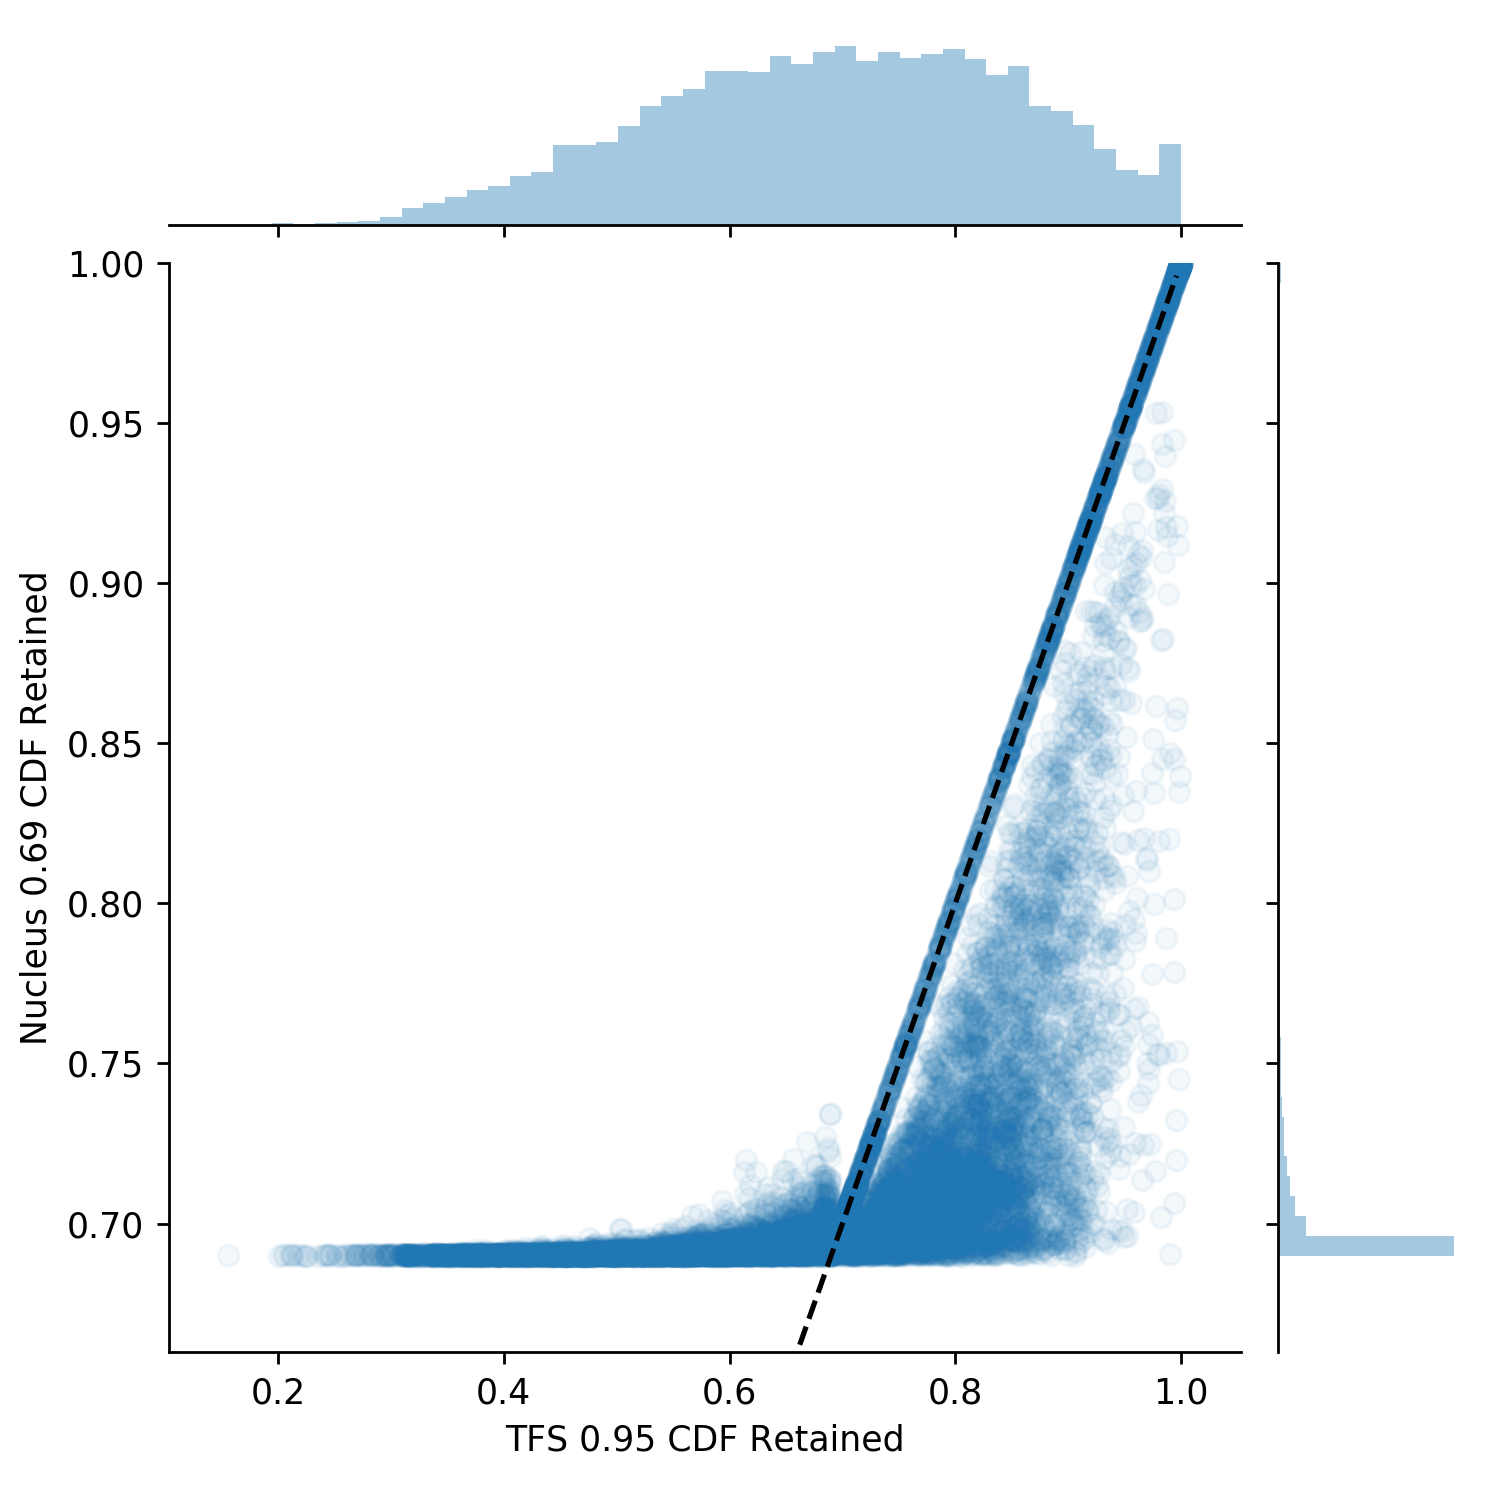
\includegraphics[width=0.95\linewidth]{figures/TFS_nineFive_vs_Nuc_sixNine_CDF_Plot.png} 
	    \caption{The Nucleus CDF deviates from its set 0.69 point when the smallest set of tokens surpasses the cutoff.}
	    \end{subfigure}
	    
	    \begin{subfigure}{0.5\textwidth}
	    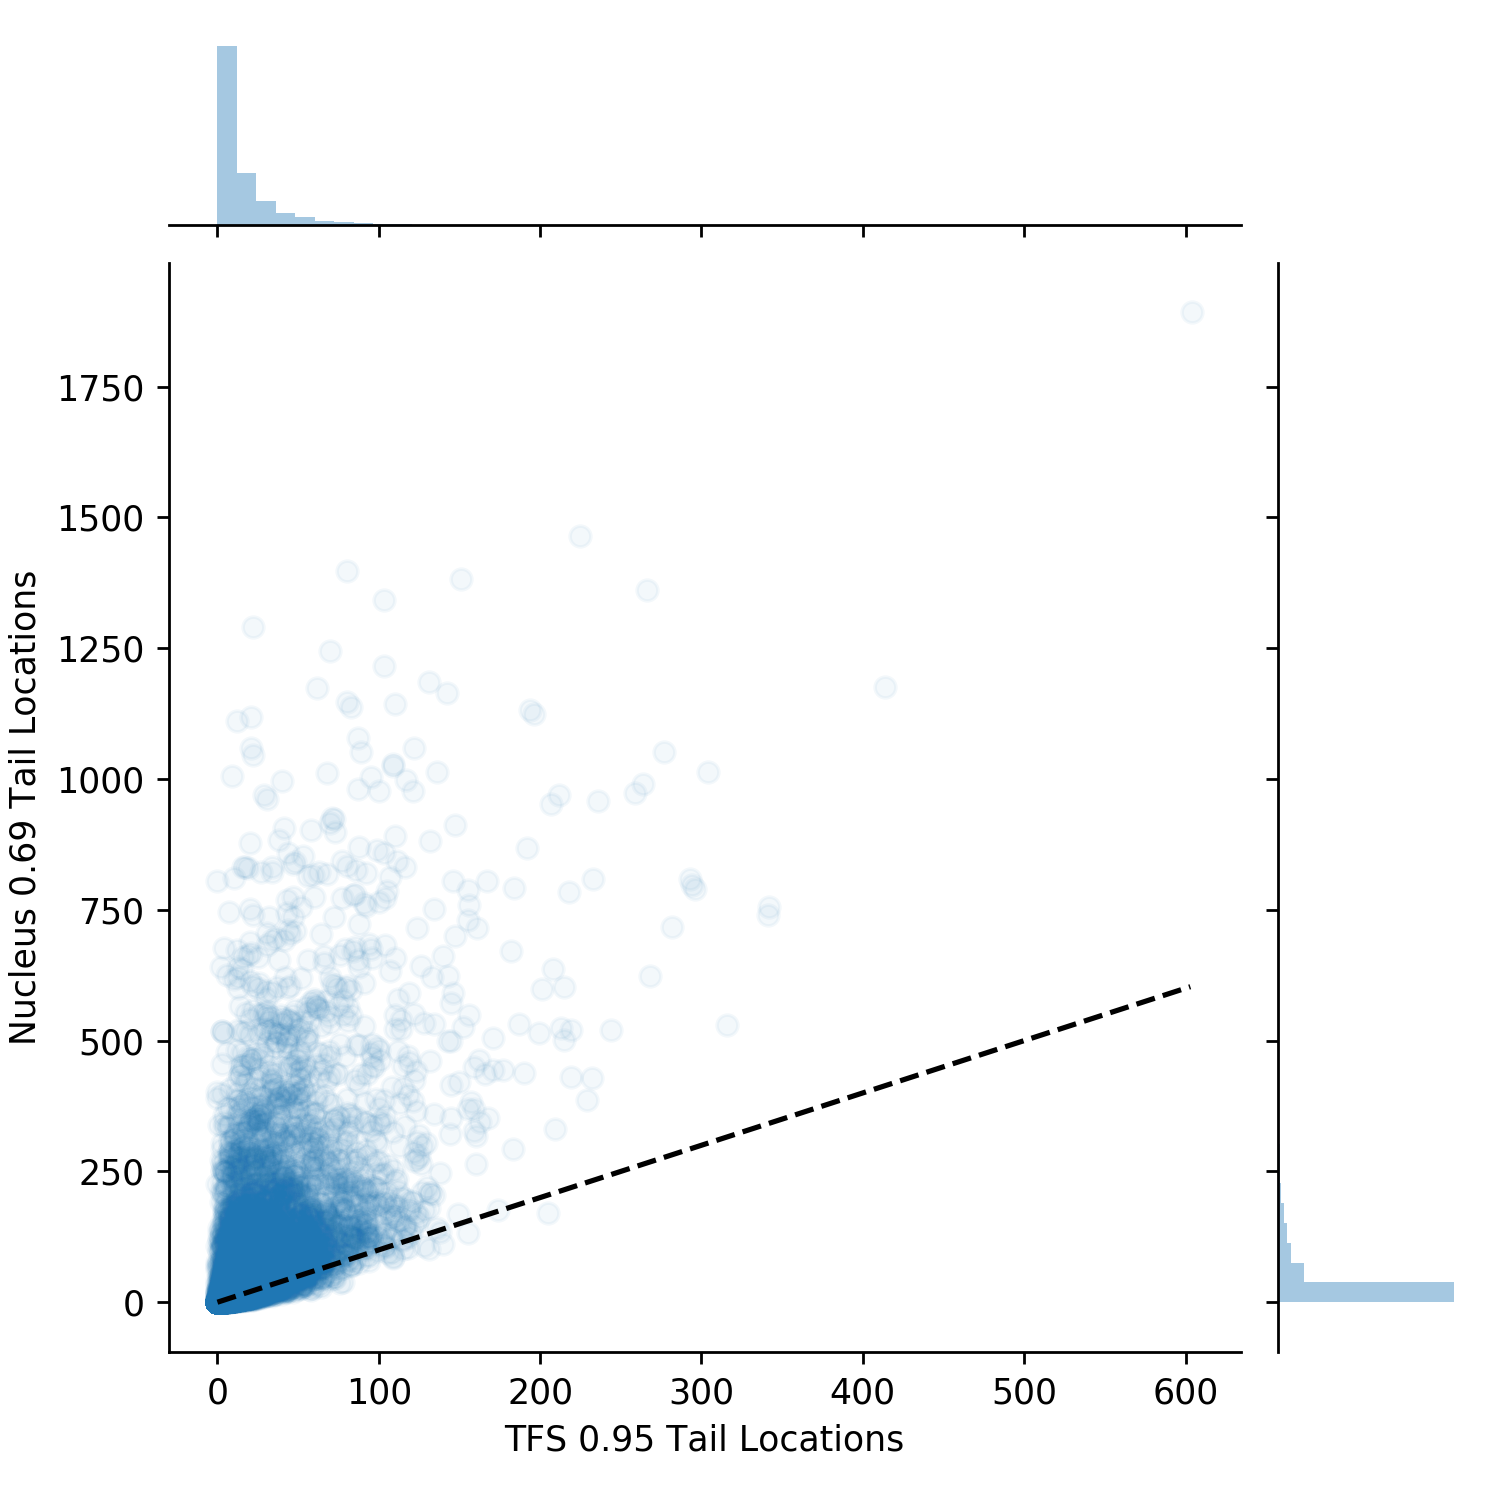
\includegraphics[width=0.95\linewidth]{figures/TFS_nineFive_vs_Nuc_sixNine_ID_Plot.png}
	    %, height=5cm
	    \caption{TFS having a tighter tail for the same token probability distributions is shown clearly here.}
	    \end{subfigure}
 
	\caption{The CDF retained (Left) and Tail Location (Right) for TFS where $z=0.95$ against Nucleus where $p=0.69$. A black dotted line is added where $x=y$ ~15\% of the 13,800 points exist along it. This is where the token probability distribution is very tight with the first few or single token taking almost all of the probability, causing the TFS and Nucleus methods to agree. ~48\% of points are to the left of $x=y$ and ~38\% to the right. Therefore, a majority of the time the TFS prunes more tightly than Nucleus leaving less of the CDF and a tighter tail location. }
	\label{fig:DiffTFSvsNucScatter}
\end{figure}

While TFS deviates from Nucleus sampling in its tail location, this is neither good or bad without looking at plots of exactly where each method draws its cutoff. This resulted in an investigation into cases of maximum deviation between the methods. The most extreme deviations exist in the bottom left and portions of the CDF plot \ref{fig:DiffTFSvsNucScatter}(a) where Nucleus behaves as it should with a CDF around 0.69 but TFS has a cut that leads to a very small or large CDF. The top ten TFS tail locations were located. Four are randomly selected and are displayed in \ref{fig:MaxDisagree} with the remainder in the Appendix.

\begin{figure}[h]
  \begin{subfigure}{.5\textwidth}
    \centering
    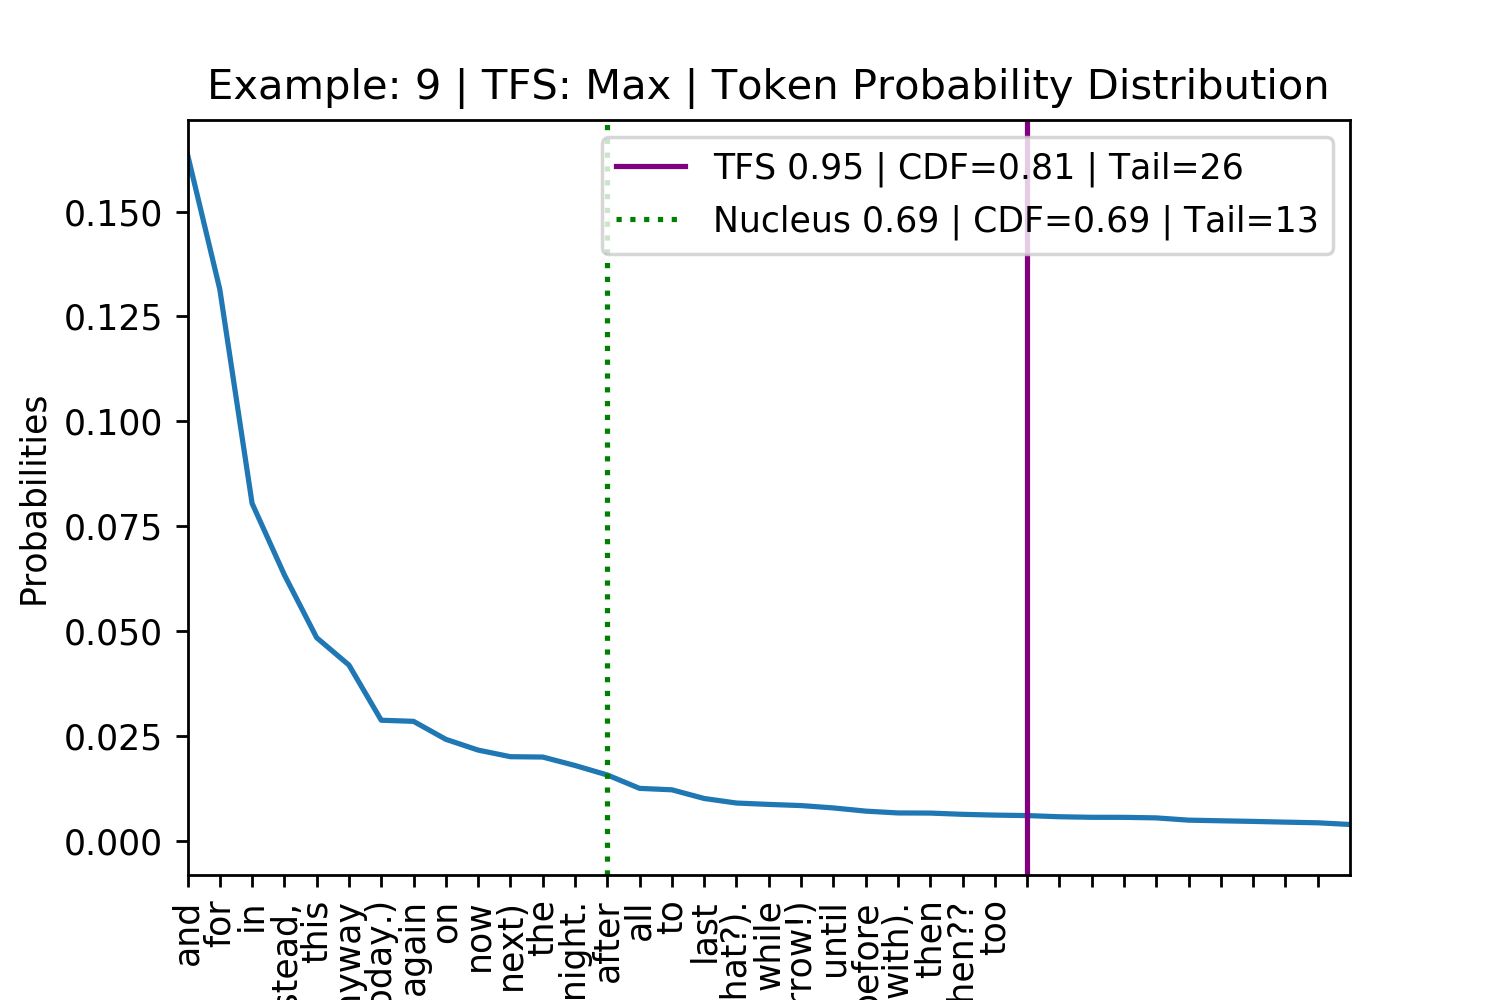
\includegraphics[width=\linewidth]{MaxDisagreement_TFS_zeroNine_Max_example-8.png}
    %\caption{Sorted Probabilities for representative logits generated from GPT-2.}
  \end{subfigure}
  \hfill
  \begin{subfigure}{.5\textwidth}
    \centering
    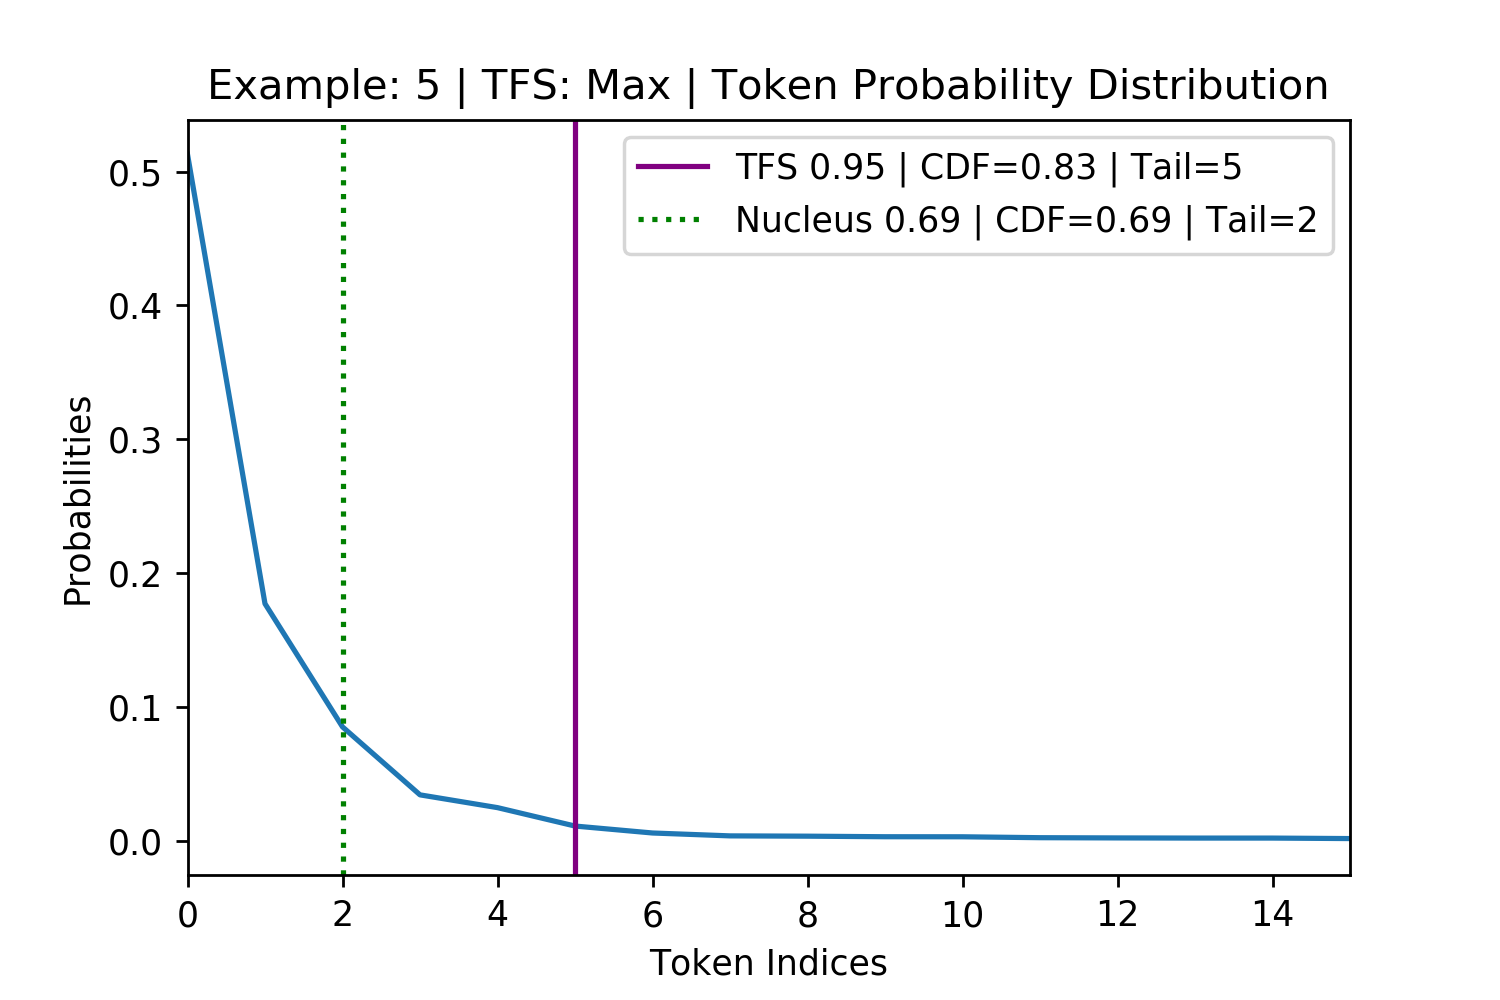
\includegraphics[width=\linewidth]{MaxDisagreement_TFS_zeroNine_Max_example-4.png}
    %\caption{The Second Derivatives of the logits.}
  \end{subfigure}

  \medskip

  \begin{subfigure}[t]{0.5\textwidth}
    \centering
    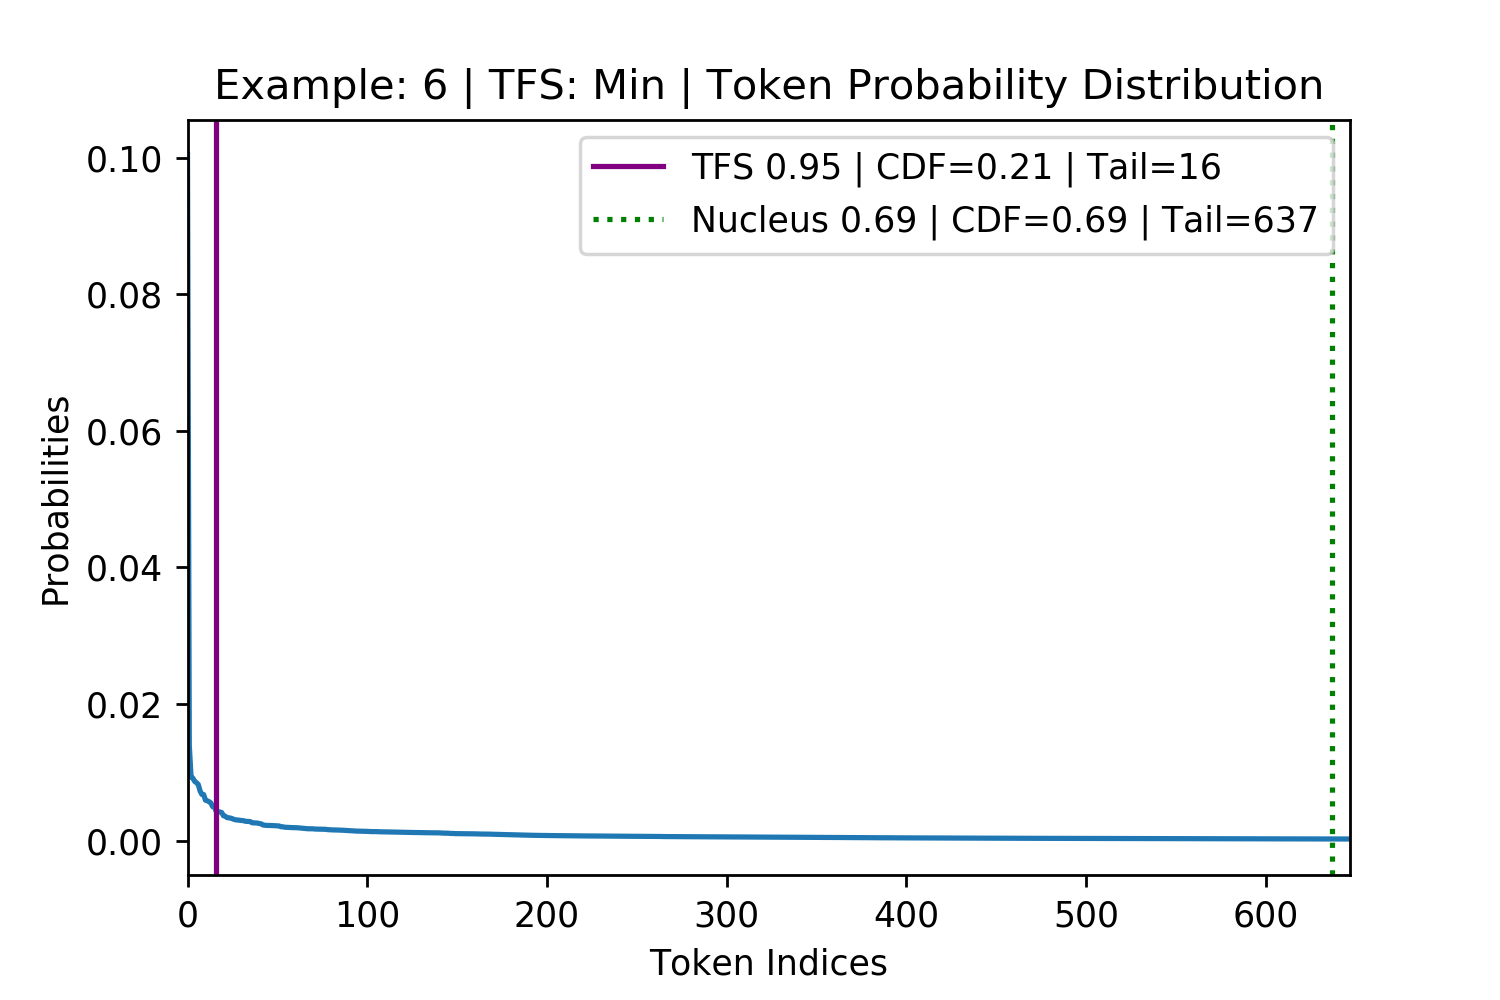
\includegraphics[width=\linewidth]{MaxDisagreement_TFS_zeroNine_Min_example-5.png}
    %\caption{The Second derivative magnitudes.}
  \end{subfigure}
  \hfill
  \begin{subfigure}[t]{0.5\textwidth}
    \centering
    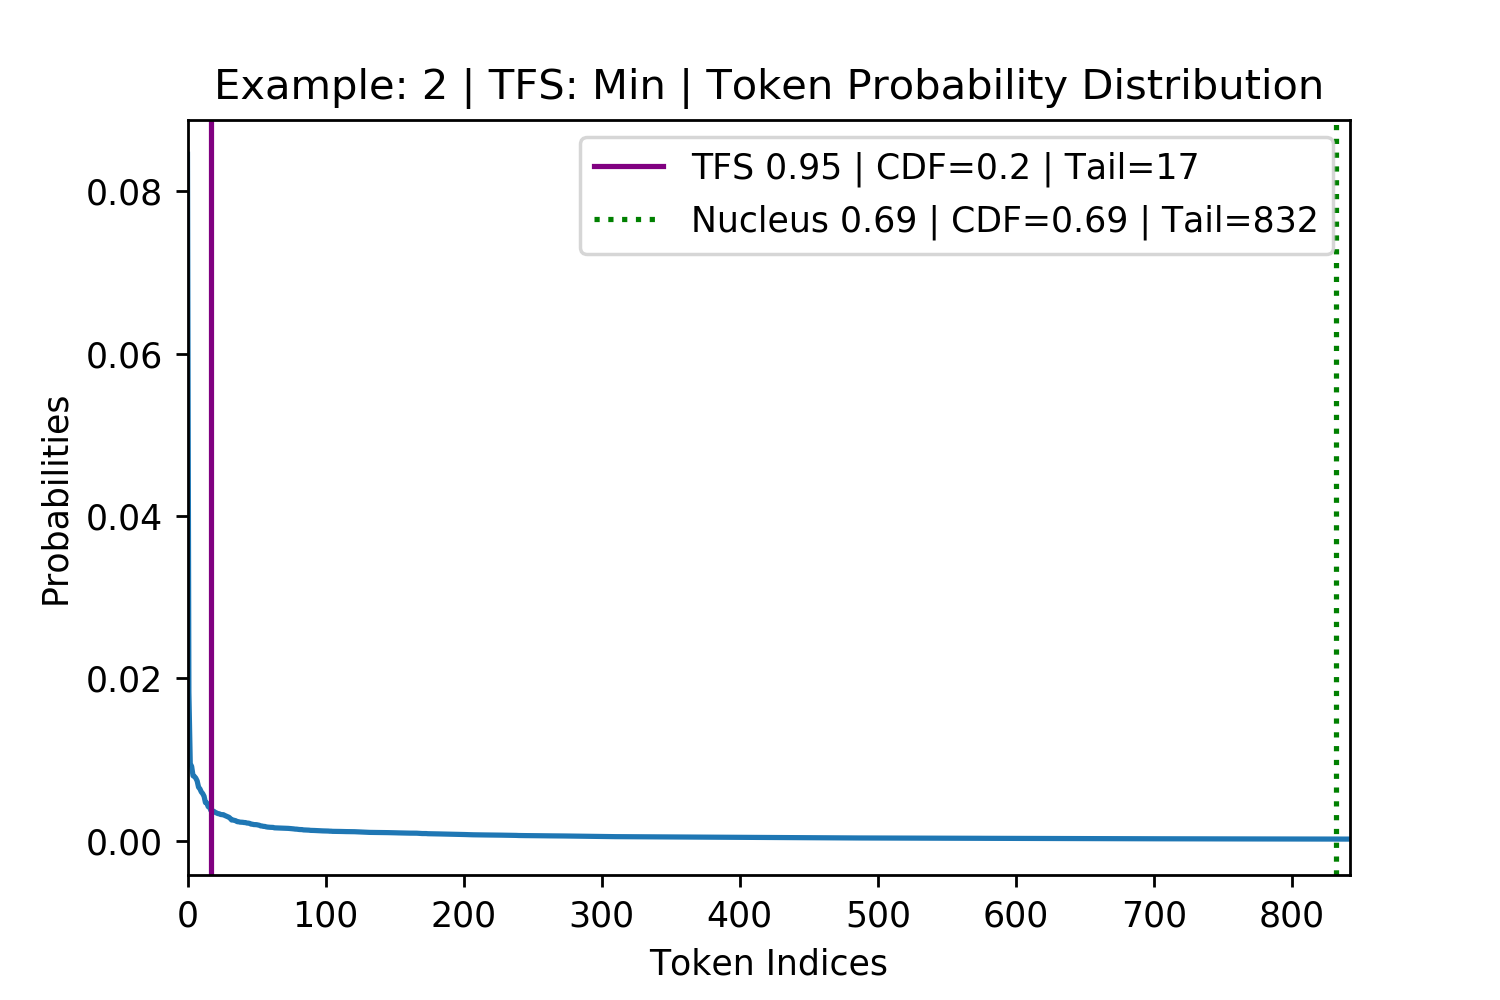
\includegraphics[width=\linewidth]{MaxDisagreement_TFS_zeroNine_Min_example-1.png}
    %\caption{The Second Derivatives cumulatively summed. A threshold is used to determine at what point to place the tail.}
  \end{subfigure}
  \caption{Four randomly selected examples of maximum disagreement between TFS and Nucleus sampling. The top row is where the TFS had the larger CDF than Nucleus (\ref{fig:DiffTFSvsNucScatter}(a) bottom right of the scatter plot). The bottom row is where the TFS had the smaller CDF than Nucleus (\ref{fig:DiffTFSvsNucScatter}(a) bottom left of the scatter plot). These examples show that Nucleus sampling's use of a fixed CDF value fails to generalize across the possible token probability distributions in finding the tail of the distribution.}
  \label{fig:MaxDisagree}
\end{figure}

This analysis of the maximum deviation between Nucleus and TFS was also helpful in ruling out another sampling method that was initially considered a simpler alternative to TFS in the form of a flat probability threshold. For example, only keeping and sampling from tokens that were above a 2\% probability. The bottom row of \ref{fig:MaxDisagree} where both of the tails are identified to be below the 2\% mark shows that such an approach would not be dynamic enough to identify the tail across different probability distributions. 

\textbf{Token Diversity} 
One validation method used by \cite{Nucleus} was to calculate the diversity of vocabulary used across all generations made by different sampling approaches in comparison to the diversity seen in the human text completions. As can be seen in \ref{fig:TokenDistributions} greedy likelihood-maximization (which is analogous to Top-K where $k=1$) has only a few words that are generated across the prompts which are repeated many times contributing to larger parts of the CDF. Meanwhile, a looser Top-K, TFS and Nucleus sampling with the investigated parameters model the human language distribution across all of the prompts quite accurately.

HERE IS WHERE GENERATING MORE SAMPLES MIGHT MAKE A DIFFERENCE. [ALSO WITH THE PERPLEXITY CI'S]

\begin{figure}[h]
    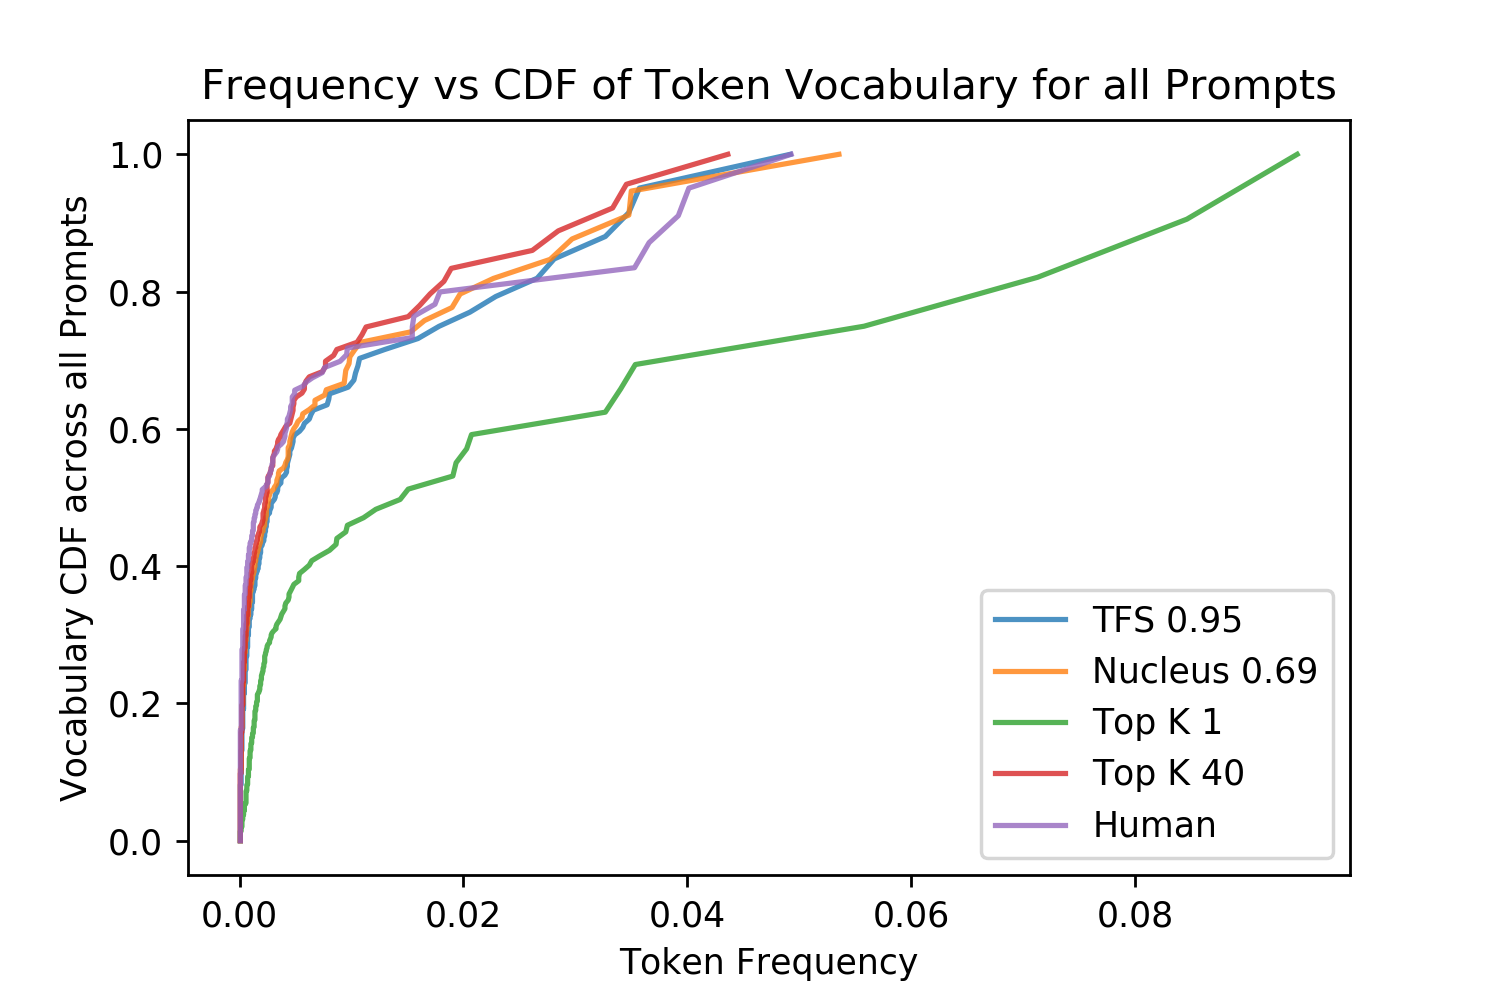
\includegraphics[width=1\textwidth]{figures/FrequencyvsCDFof_Token_onlyMainTFS_and_Nuc.png}
    \caption{Distributions of the token frequency and its contribution to the CDF. The distributions for other sampling methods can be found in the Appendix}
    \label{fig:TokenDistributions}
\end{figure}

\textbf{Model Perplexity} 
Another method that \cite{Grover} uses to evaluate sampling quality is the perplexity of model generations. Perplexity is noisy and the probabilities are all similar. Don't seem to add much. 

Need to see w/o CIs. and then with them. Need to get more examples? Need to run for longer period of time?? Run for a longer period of time and see if stabilizes over time? DO THIS FOR ONE (TFS 0.95) AND SEE WHAT HAPPENS. WILL PROBABLY WANT TO COMPUTE PERP ETC ON THE FLY? DO THIS BUT ADD IT TO Appenix FOR NOW? 

RELATE GLTR PAPER TO ENTROPY. 

\textbf{Efficiency} A potential limitation of TFS is that it is a more complex algorithm than Nucleus or Top-K sampling. In particular, the operations of both of these other sampling approaches are a subset of the TFS algorithm's mathematical operations. To evaluate differences in speed, the sampling strategies across all sampling parameters were run across all 100 prompts with 150 tokens generated for each in batches of 25. This was replicated five times using a different random seed each time so that different prompts and tokens were selected. The start and end of the batch generations of the 150 tokens was timed and compared for each method, shown in \ref{fig:MeanTimes}. At $\alpha=0.05$ there is no statistically significant difference between the sampling strategies except for Top K sampling. We hypothesize that this is because Top K sampling was already implemented in the GPT-2 source code by \cite{radford2019language} and is vectorized. None of the other implementations are currently vectorized and use a for loop to iterate through the batch. While TFS is a more complex algorithm, uniquely needing to compute the second derivative, take its absolute value, and normalize it, these operations appear to be highly efficient on a GPU \footnote{A single NVIDIA T4 GPU was used for all of the research} and result in no statistically significant speed reductions. 

RERUN TOPK WHERE I ALSO USE A FOR LOOP FOR IT. OR VECTORIZE ALL OF THE OTHERS. ENSURE THAT FLAT ISNT IN THE PLOT. 

\begin{figure}[h]
    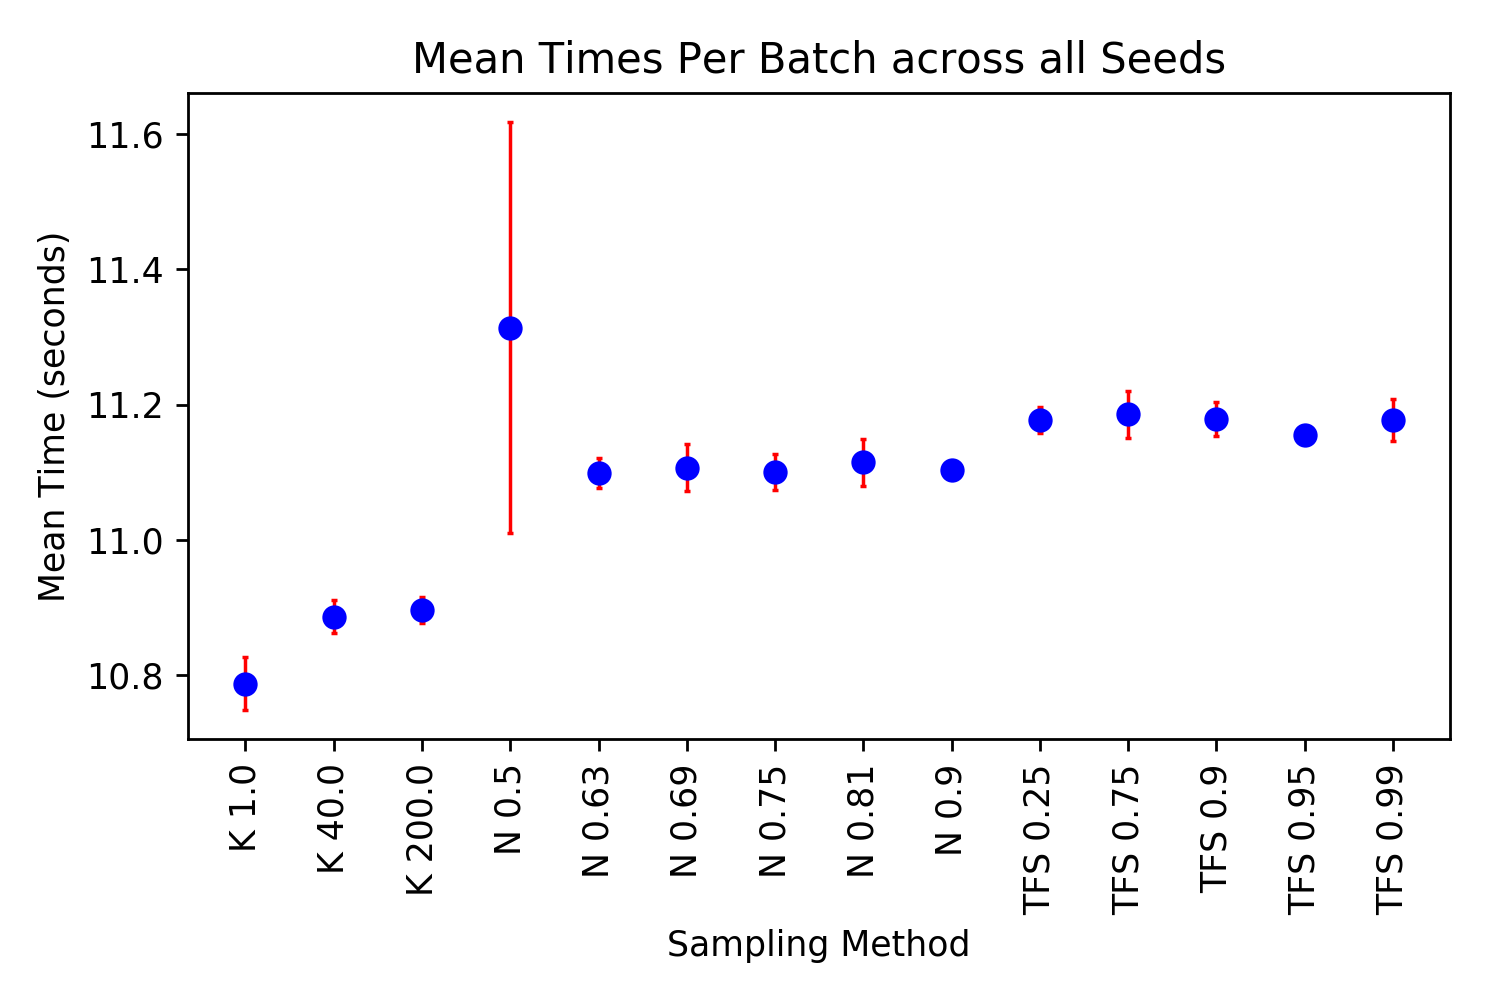
\includegraphics[width=1\textwidth]{figures/MeanTimesPerBatch.png}
    \caption{Average times taken to generate a batch of 25, 150 token long outputs. 95\% Confidence Intervals provided}
    \label{fig:MeanTimes}
\end{figure}

\textbf{Human Evaluation} 
The terminal goal of any language generation task is to produce text that humans rate to be of a high quality while also maintaining diversity. \cite{Nucleus} failed to perform any human evaluation of Nucleus sampling against Top-K sampling so to the authors knowledge these existing methods are compared with each other and also TFS using human evaluators. The evaluators were crowdsourced from Amazon Mechanical Turk CITE THE WEBSITE and were tasked with determining which of two text generations for a given prompt was better in quality. ADD IN ALL OTHER DETAILS INCLUDING IF IT WAS FROM GROVER OR NOT. 

\section{Future Work} PROBABLY GET RID OF THIS
While there are likely to be a number of different independent reasons why likelihood-maximization fails to produce high quality outputs on open-ended generation tasks and progress has been made in addressing it. For example, by penalizing the model during training for assigning a high probability to previous words (\cite{UnLikelihood}) and using stochastic sampling that restricts the space of possible outputs (\cite{Nucleus}), the fact that a powerful auto-regressive model like GPT-2 (\cite{radford2019language}), after generating a sentence like "I don't know", decides that the next sequence of words of highest probability is to again repeat the phrase, "I don't know"\footnote{This very example of a model repeating "I don't know" again and again with increasingly probability assigned to the repeating sentence has been observed in \cite{Nucleus}} suggests that a larger problem with our models is to correctly condition them on the given task or prompt. When a human speaks a sentence (most of the time) they know what the meta-level point is and how their sentence is going to end. Novel network architectures like XLNet (\cite{XLNet}), which is auto-regressive but can be conditioned on the past and future parts of a sequence may provide one solution but there are certainly others also worthy of future exploration. 

\section{Conclusion}

In this paper we present Tail Free sampling, a new method to sample from neural networks for open-ended generation tasks. Our method is motivated by finding the subset of a vocabulary that is exchangeable in a given context and does so by finding where the model (which hopefully matches reality) plateaus in the probability assigned to its tokens. We should that existing approaches fail to achieve the same objective and as a consequence do not peform as well in human evaluations of text generation. In addition, this approach is computationally efficient and can generalize across problem domains and model vocabulary sizes where existing methods could not.

SHOULD AUTHORS BE PLURAL?
\section*{Acknowledgements} 
DOUBLE CHECK AUTHORS ARENT IN ACKNOWLEDGEMENTS!?
The authors would David Banks, Miles Turpin, Nathan Rollins, Debora Marks, Elle Deich, Gwern Branwen without whose commentary, feedback, and inspiration this work would not have been possible. Funding for this project was provided indirectly through Daniel Bricken, the Robertson Scholars Leadership Program, and the Google Cloud Platform's free trial credits.

\bibliographystyle{plainnat}
\bibliography{references}
%\bibliographystyle{unsrt}  
%%% Remove comment to use the external .bib file (using bibtex).
%%% and comment out the ``thebibliography'' section.

\section*{Appendix}

CITE NUMPY, PANDAS, SCIPY, MATPLOTLIB, SEABORN, TENSORFLOW, ANACONDA/JUPYTERNOTEBOOKS(?), AND THANK ALL THE OPEN SOURCE CONTRIBUTORS. 

Also need to add the other examples of the tails found and the max disagreements. 

\section{Headings: first level}
\label{sec:headings}

\lipsum[4] See Section \ref{sec:headings}.

\subsection{Headings: second level}
\lipsum[5]
\begin{equation}
\xi _{ij}(t)=P(x_{t}=i,x_{t+1}=j|y,v,w;\theta)= {\frac {\alpha _{i}(t)a^{w_t}_{ij}\beta _{j}(t+1)b^{v_{t+1}}_{j}(y_{t+1})}{\sum _{i=1}^{N} \sum _{j=1}^{N} \alpha _{i}(t)a^{w_t}_{ij}\beta _{j}(t+1)b^{v_{t+1}}_{j}(y_{t+1})}}
\end{equation}

\subsubsection{Headings: third level}
\lipsum[6]

\paragraph{Paragraph}
\lipsum[7]

\section{Examples of citations, figures, tables, references}
\label{sec:others}
\lipsum[8] \cite{kour2014real,kour2014fast} and see \cite{hadash2018estimate}.

The documentation for \verb+natbib+ may be found at
\begin{center}
  \url{http://mirrors.ctan.org/macros/latex/contrib/natbib/natnotes.pdf}
\end{center}
Of note is the command \verb+\citet+, which produces citations
appropriate for use in inline text.  For example,
\begin{verbatim}
   \citet{hasselmo} investigated\dots
\end{verbatim}
produces
\begin{quote}
  Hasselmo, et al.\ (1995) investigated\dots
\end{quote}

\begin{center}
  \url{https://www.ctan.org/pkg/booktabs}
\end{center}

\subsection{Tables}
\lipsum[12]
See awesome Table~\ref{tab:table}.

\begin{table}
 \caption{Sample table title}
  \centering
  \begin{tabular}{lll}
    \toprule
    \multicolumn{2}{c}{Part}                   \\
    \cmidrule(r){1-2}
    Name     & Description     & Size ($\mu$m) \\
    \midrule
    Dendrite & Input terminal  & $\sim$100     \\
    Axon     & Output terminal & $\sim$10      \\
    Soma     & Cell body       & up to $10^6$  \\
    \bottomrule
  \end{tabular}
  \label{tab:table}
\end{table}

\subsection{Lists}
\begin{itemize}
\item Lorem ipsum dolor sit amet
\item consectetur adipiscing elit. 
\item Aliquam dignissim blandit est, in dictum tortor gravida eget. In ac rutrum magna.
\end{itemize}


\end{document}

